% -*- TeX:SI -*-
% slovene sub-mode for spell check

%\Large\textbf
\chapter{{KUKA Youbot mobilna platforma}}

\vspace{-1.5cm}

\begin{mdframed}[backgroundcolor=green!20, shadow=true,roundcorner=8pt]
\vspace{-0.35cm}
\section{Cilji vaje}
\begin{itemize}
\item spoznavanje z vodenjem mobilne platforme youBot Kuka
\item uporaba znanja pridobljenega na predavanjih o homogenih transformacijah med različnimi koordinatnimi sistemi
\item uporaba video sistema za vodenje mobilne robotske platforme
\item spoznavanje okolja Matlab Simulink za preračun homogenih transformacij, vodenje platforme in načrtanje posameznih korakov za izvedbo večstopenjeske naloga pobiranja in prenašanja različnih objektov


\end{itemize}
\end{mdframed}



\section{Uvod}
 Industrijska robotika je v stalnem porastu in še za vrsto let vnaprej lahko rečemo, da bo vsako novo leto tudi leto z novim porastom števila industrijskih robotskih aplikacij in nameščenih robotov v industrijskem okolju. Nameščeni oziroma pričvrščeni na svoje mesto v proizvodnem procesu so sposobni opravljati naloge, ki zahtevajo natančnost in hitro izvajanja ciklov. Precejšen del industrije je močno odvisen od industrijskih robotov. Kljub temu pa imajo eno bistveno pomanjkljivost, in to je pomanjkanje mobilnosti. Pritrjen manipulator ima omejen delovni prostor, ki je določen s kinematično strukturo roke in seveda z mestom kjer je pritrjen. Mobilni roboti imajo seveda to prednost, da se lahko pomikajo po prostoru in je njihov delovni prostor precej manj omejen in veliko večji. Seveda pa se s tem odpre celo novo področje vodenja robotov, kjer je glavni problem določanje lege robota v prostoru. če je za določenje lege robota v prostoru v primeru industrijskih robotov dovolj en enkoder v vsakem sklepu, pa je za določanje lege v prostoru pri mobilnih robotih potrebno imeti na voljo večje število senzorjev.

Mobilni roboti odpirajo celo vrsto novih možnosti in postajo zanimivi tudi za industrijsko okolje, še mnogo bolj zanimivi pa za okolje v katerem se gibljemo tudi mi sami, dasiravno ima človeška domišljija močno nerealna pričakovanja česa vse naj bi bili mobilni roboti sposobni.
KUKA youBot je mobilna platforma z robotsko roko, ki jo je razvilo nemško podjetje KUKA, ki izdeluje industrijske robote.

KUKA youBot je namenjen za izobraževanje in raziskave na področju mobilne robotike. Zaradi tega se KUKA youBot ponaša z odprto krmilniško arhitekturo, kar omogoča dostop do vseh nivojev strojne opreme in vodenja. Delo s KUKA youBot-om torej zahtevo vsaj osnovno znanje iz robotike in vodenja naprav, kar je seveda nadvse primerno za uporabo KUKA youBot platforme pri vajah pri predmetu Osnove robotike.
KUKA youBot je sestavljena iz dveh poglavitnih delov:
\begin{itemize}
\item KUKA youBot vsesmerna mobilna platforma (ang. omni-directional mobile platform) je sestavljena iz ohišja, štirih vsesmernih švedskih koles (ang. mecanum wheels), štirih motorjev za pogon koles, osebnega računalnika in seveda potrebnih elektronskih vezij. Uporabniki lahko bodisi zaganjajo algoritme vodenja na računalniku, ki se nahaja na platformi, ali pa na oddaljenem računalniku.
\item KUKA youBot antropomorfna robotska roka ima 5 prostostnih stopenj in dvoprstno prijemalo. če je robotska roka nameščnea na mobilno platformo, vodenje roke poteka prek računalnika na mobilni platformi. Roko je možno voditi tudi brez platforme z navadnim osebnim računalnikom preko Ethernet povezave.
\end{itemize}

Na platformo je mogoče montirati še vrsto senzorjev kot so Kinect 3D Camera, laserski merilec razdalje, stereo kamero, ultrazvočne merilnike razdalje, itd.

\section{Hiter pregled vaje}

Pri tej vaji boste s pomočjo KUKA youBot platforme, ki je prikazana na sliki \ref{fig:KUKA1}, igrali miselno igro Hanojski stolp.

\emph{Hanojski stolp} je miselna oziroma logična igra. Začne se s stolpom diskov, ki so naloženi na drug drugega od največjega spodaj do najmanjšega zgoraj, kot je prikazano na sliki \ref{fig:han_tower}. Cilj je prenesti diske na drugo mesto, kjer morajo biti postavljeni v istem vrstnem redu, pri čemer imamo na voljo samo eno vmesno odlagališče. Pri reševanju moramo upoštevati naslednja pravila:

\begin{itemize}
\item Diske premikamo posamično.
\item Poteza zajema premik zgornjega diska na drugo mesto oziroma premik na večji disk.
\item Nikdar ne smemo postaviti večjega diska na vrh manjšega diska.
\end{itemize}

\begin{figure}[h]
\centering \resizebox{6cm}{!}{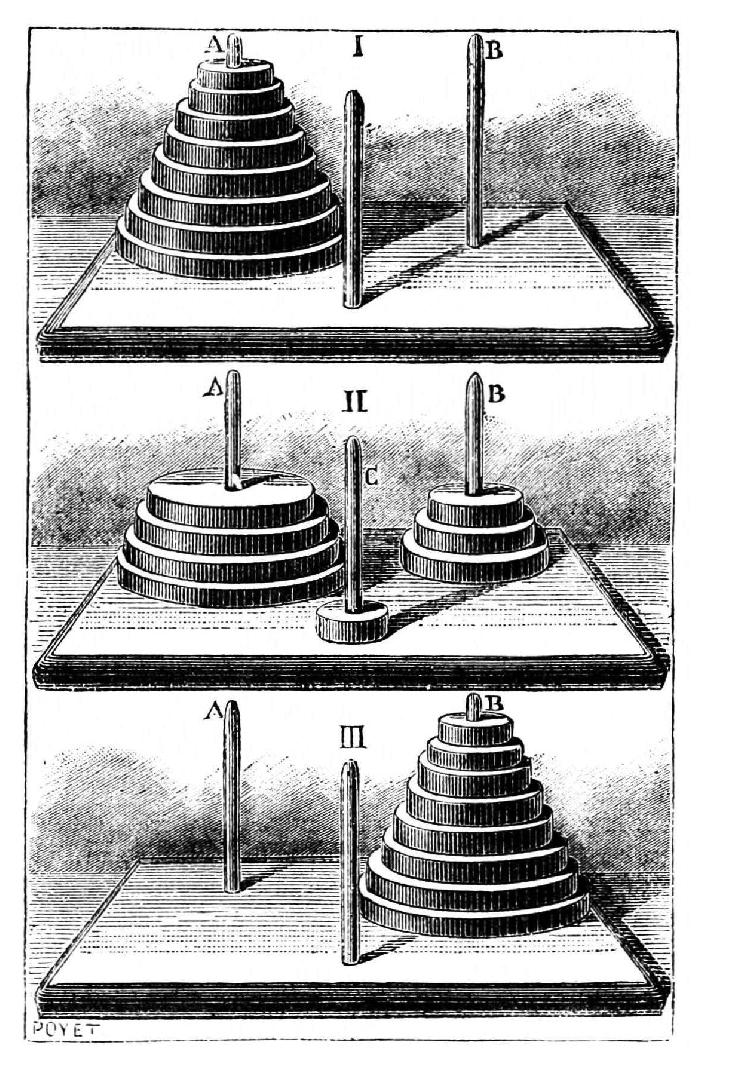
\includegraphics[draft=false]{PSM_V26_D464_The_tower_of_hanoi.eps}}
\caption{Igra Hanojski stolp z diski različnih velikosti.}
\label{fig:han_tower}
\end{figure}

Za reševanje igre z robotom se namesto diskov uporabja kocke. Med seboj se razlikujejo po barvi vrhnje kocke, ki je namenjen za prijem. Vse kocke so enako velike, največji disk prestavljajo tri rumene kocke, naslednji disk dve rdeči kocki, najmanjši disk pa ena zelena kocka. Igro se torej igra kot bi imel tri diske različnih velikosti.

Za izvedbo naloge uporabljamo tri lokacije, začetna lokacija kock, vmesno odlagališče, ter končna lokacija. Začetno postavitev naloge prikazujeta sliki \ref{fig:AllFrames} in \ref{fig:AllTocke}. Cilj naloge je, da s pomočjo robota prestavimo kocke iz začetne na končno lokacijo po naslednjih pravilih: barvne oznake so zelena, rdeča in rumena. Rumenih kock ne smemo nikoli postaviti pred rdečimi oziroma zelenimi kockami, pravtako  rdečih kock ne smemo nikoli prstaviti pred zelenimi. Vedno smemo prestavljati samo kocke ene barve, ker predstavljajo en disk, v vrsti morajo seveda ležati le kocke istih barv.  Pravilni vrstni red postavitve je prikazan na slikah \ref{fig:AllFrames} in \ref{fig:AllTocke}.

Koraki za izvedbo naloge so sledeči:
\begin{enumerate}
\item Pretvorba iz koordinatnega sistema kamere v globalni koordinatni sistem.
    \begin{enumerate}
    \item Odprava perspektive pri zajemanju pozicije objektov s pomočjo kamere.
    \item Transformacija leg objektov iz koordinatnega sistema kamere v globalni koordinatni sistem.
    \end{enumerate}
\item Priprava preprostega regulatorja za vodenje mobilne platforme v globalnem koordinatnem sistemu.
\item Programiranje zaporedja operacij za nalogo "Hanojski stolp".

\end{enumerate}


\section{KUKA youBot vsesmerna mobilna platforma}

KUKA youBot platforma je vsesmerna mobilna platforma s štirimi švedskimi kolesi. Vsesmerno gibanje ji mogočajo švedska kolesa (poimenovana po narodnosti izumitelja teh koles Bengta Ilona, v literaturi so pogosto imenovana tudi Mecanum kolesa), vsako kolo ima svoj motor. Platforma se tako lahko giblje naprej-nazaj, levo-desno in rotira okoli svoje osi. Platforma ima torej 3 prostostne stopnje.
Slika 1 prikazuje koordinatni sistem na KUKA youBot vsesmerni mobilni platformi. Os x kaže v smeri naprej (na sprednjem delu platform je pritrjena robotska roka, na zadnjem delu pa je nameščena miza za odlaganje predmetov), y os kaže v smeri levo, z os pa navzgor. \vspace{1cm}

\begin{figure}[h]
\centering \resizebox{10cm}{!}{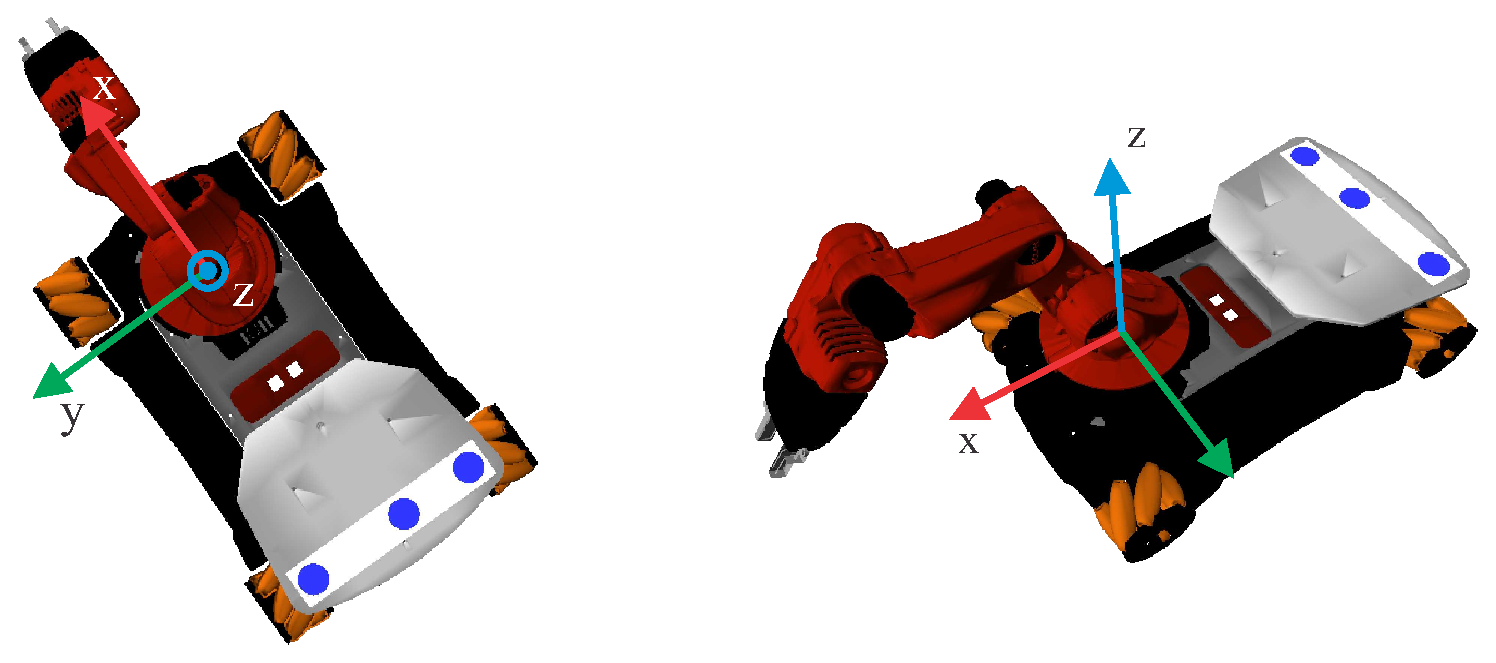
\includegraphics[draft=false]{KUKAFrame-4.eps}}
\caption{KUKA youBot s koordinatnim sistemom.}
\label{fig:KUKA1}
\end{figure}

Platformo vodimo tako, da podamo vektor treh hitrosti $\begin{bmatrix} v_x \\ v_y \\ \omega_z \end{bmatrix}$:
\begin{itemize}
\item hitrost gibanja v $x$ smeri $v_x$,
\item hitrost gibanja v $y$ smeri $v_y$,
\item hitrost rotiranja okoli $z$ osu $\omega_z$.
\end{itemize}
Platforma sama ne vsebuje nobenih senzorjev, ki bi omogočali določanjene njene lege v prostoru. Za določanje lege platforme v prostoru se uporablja kamero, ki je nameščena na stropu. Z robotskim vidom je tako mogoče določiti lego platforme v prostoru. Več o tem je zapisano v podpoglavju \ref{pog:RobVid}.

\section{KUKA youBot robotska roka}

KUKA youBot robotska roka je serijski mehanizem s petimi prostostnimi stopnjami. Na koncu prijemala se nahaj dvoprstno prijemalo. Roka ima v sklepih enkoderje za merjenje kota zasuka v sklepu, vsak sklep poganjajo električni motorji, ki nima mehanskih zavor. če torej izklopimo napajanje na platformi, se bo robotska roka sesedla. Roka lahko dvigne $0.5$ $kg$ in ima dosega v horizontalni ravnini $0.54$ $m$. Koordinatni sistem platforme je namerno postavljen pod bazo robotske roke, saj se tako bazni koordinatni sistem robotske roke in platforme pokrivata. Koordinatna sistema platforme in roke sta torej ista.

\vspace{0.5cm}

\begin{table}
\caption{Lastnosti KUKA youBot robotske roke}
\begin{tabular}{|l|l|}
\hline Krmiljene osi & 5 \\
\hline Nosilnost &	0,5 kg \\
\hline Doseg &	540 mm \\
\hline Ponovljivost & 	1 mm \\ \hline
\end{tabular}
\end{table}

%\vspace{0.5cm}

\begin{table}
\caption{Obseg gibanja za posamezni sklep}
\begin{tabular}{|l|l|}
\hline Os i & $\Theta_i$ \\
\hline 1 &	+/- 169$\,^{\circ}$ \\
\hline 2 &	+90 $\,^{\circ}$/-65 $\,^{\circ}$ \\
\hline 3 & 	+146 $\,^{\circ}$/-151 $\,^{\circ}$ \\
\hline 4 & 	+/-102 $ \,^{\circ}$ \\
\hline 5 & 	+/-167 $ \,^{\circ}$ \\ \hline
\end{tabular}
\end{table}

\vspace{0.5cm}

\begin{figure}[h]
\centering \resizebox{10cm}{!}{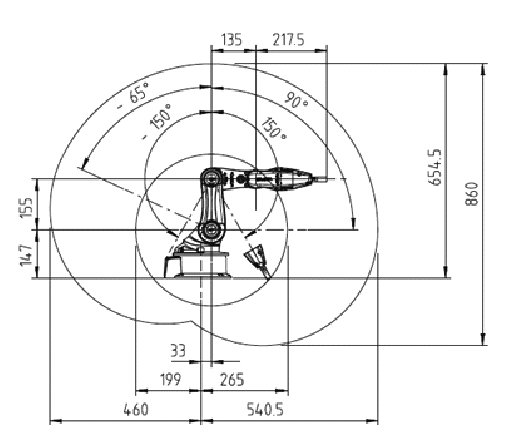
\includegraphics[draft=false]{envelope.eps}}
\caption{Delovni prostor roke youBot.}
\end{figure}

Robotsko roko vodimo s pomočjo inverzne kinematike, ki je v sheme vodenja že vključena. Vhod v inverzno kinematiko je vektor 5 vrednosti (glej sliko \ref{fig:RokaKoor}):
\begin{itemize}
\item vektor treh vrednosti $x$, $y$, $z$, ki predstavljajo željeno pozicijo vrha v koordinatnem sistemu platforme,
\item kot $\theta$, ki predstavlja kot zasuka predzadnjega segmenta robotske roke,
\item zapri/odpri prijemalo.
\end{itemize}

\begin{figure}[h]
\psfrag{th}[][l][3.0][0]{$\theta$}
\psfrag{p}[][l][3.0][0]{$p$}
\psfrag{x}[][l][3.0][0]{$x$}
\psfrag{y}[][l][3.0][0]{$y$}
\psfrag{z}[][l][3.0][0]{$z$}
\centering \resizebox{10cm}{!}{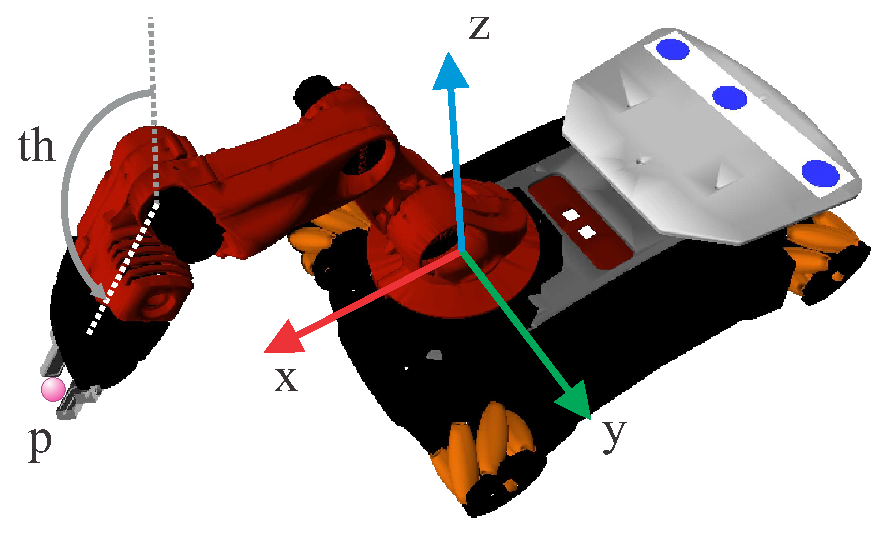
\includegraphics[draft=false]{KUKAFrame-3.eps}}
\caption{Robotksa roka KUKA. Točka $p$ predstavlja točko pomika vrha roke v koordinatnem sistemu platforme, kot $\theta$ pa zasuka predzadnjega segmenta roke.}
\label{fig:RokaKoor}
\end{figure}


\section{Robotski vid za določanje lege platforme}\label{pog:RobVid}

Za zajem slike se uporablja spletno kamero Logitech HD C920, ki omogoča zajem videa z ločljivostjo 1280x720 slikovnih pik (ang. pixel) in široki kot pogleda $85$ stopinj. Kamera je nameščena na višino $2.81$ metra, kar omogoča vidno polje $3.84$ x $2.16$ metra. To je torej delovni prostor platforme.
Zajeta slika se obdela v programskem okolju MATLAB z orodjem Image Processing Toolbox. Orodje Image Acquisition Toolbox omogoča direktni dostop do kamere in s tem tudi zajem videa oziroma posameznih slik.


\begin{figure}[h]
\psfrag{x}[][l][2.0][0]{$x_C$}
\psfrag{y}[][l][2.0][0]{$y_C$}
\psfrag{z}[][l][2.0][0]{$z_C$}
\centering \resizebox{10cm}{!}{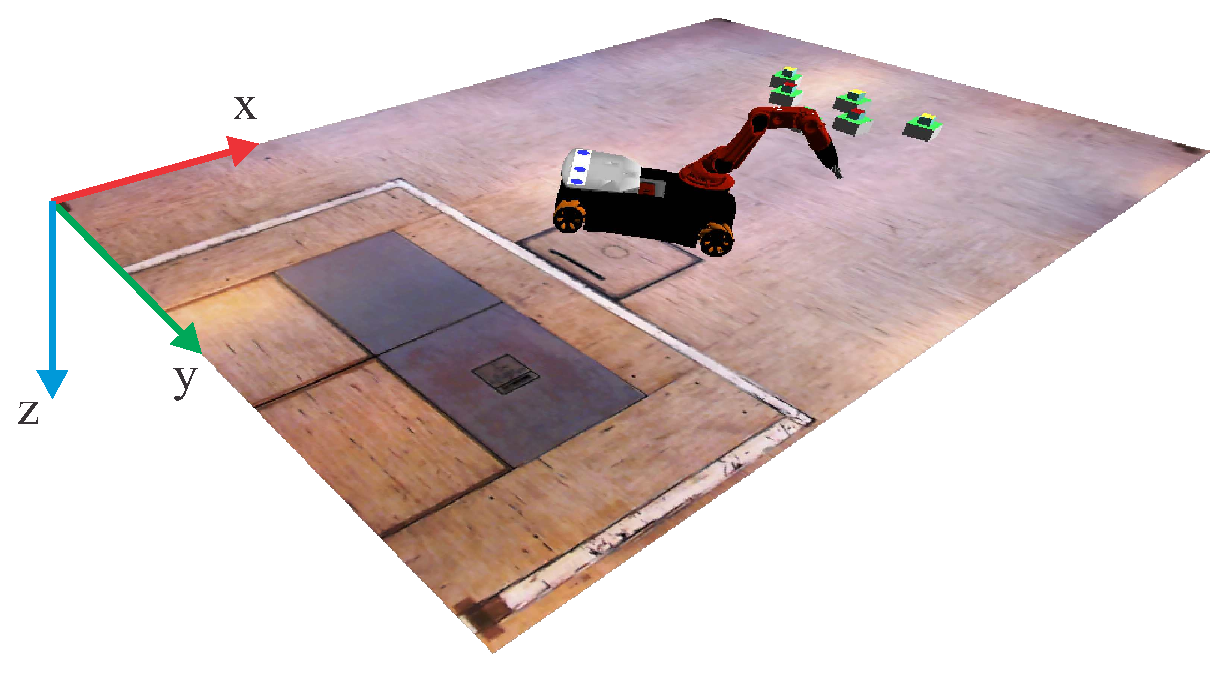
\includegraphics[draft=false]{cameraFrame.eps}}
\caption{Vidno polje kamere, ki določa delovni prostor platforme, in koordinatni sistem kamere.}
\end{figure}

Program za obdelavo slike je namenjen iskanju lege platforme in začetne lege 6 kock. Vrača $x$ in $y$ koordinato ter kot zasuka $\varphi$ za platformo in vsako od 6 kock. Na platformi se na plošči za odlaganje nahajajo tri modre pike iz katerih program za obdelavo slike določi pozicijo in orientacijo platforme. Program izračunava novo pozicijo platforme s 10 osvežitvami lege na sekundo (ang. 10 FPS), medtem ko se lego kock določi samo enkrat na začetku. Program vrača koordinati $x$ in $y$, ki sta že preračunani v metre v koordinatnem sistemu kamere. Za platformo tudi že vrača pozicijo izhodišča koordinatnega sistemom na KUKA platformi. Program najprej določi položaj posameznih treh pik, izračuna sredinsko lego med skrajnima modrima točkama in doda premik do koordnatnega sistema platfome. Kot $\varphi$ določa kot med x-osjo koordinatnega sistema kamere in x-osjo koordinatnega sistema platforme.

\begin{figure}[h]
\psfrag{x1}[][l][2.0][0]{$x_C$}
\psfrag{y1}[][l][2.0][0]{$y_C$}
\psfrag{z1}[][l][2.0][0]{$z_C$}
\psfrag{x3}[][l][2.0][0]{\color{white}$x_K$}
\psfrag{y3}[][l][2.0][0]{\color{white}$y_K$}
\psfrag{z3}[][l][2.0][0]{\color{white}$z_K$}
\psfrag{fi}[][l][2.0][0]{\color{white}$\varphi$}
\psfrag{[xK,yK]}[][r][2.0][0]{\color{white}$[\prescript{C}{}x_K,\,\,\prescript{C}{}y_K]$}
\centering \resizebox{10cm}{!}{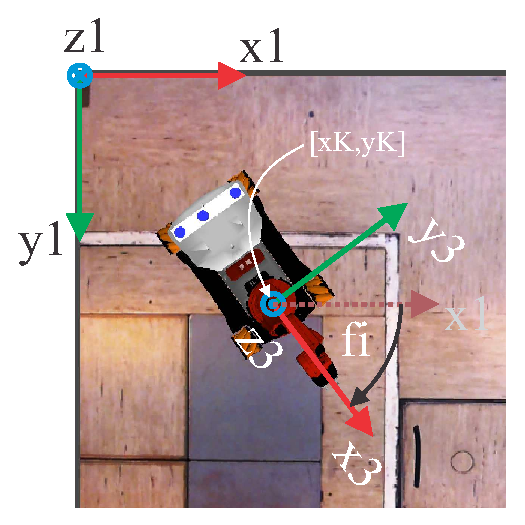
\includegraphics[draft=false]{frames-3.eps}}
\caption{Koordinatni sistem kamere cs1 in koordinatni sistem KUKE cs3.}
\end{figure}

\section{Zapis leg platforme in roke}

Kljub temu, da sta koordinatna sistema roke in platforme postavljena na isti mesti, pa se zapisa leg platforme in roke razlikujeta. Ker se platforma premika v ravnini, se za zapis pozicije platforme uporablja dve koordinati in sicer $x$ in $y$ pozicijo platforme. Platformi lahko orientacijo spreminjamo samo okoli z osi, zato za orientacijo platforme zadostuje en kot $\varphi$. Lega platforme je torej zapisana z dvema podatkoma za pozicijo ter enim za orientacijo. Lego torej zapišemo z vektorjem $[x_K, y_K, \varphi]$.
Pri robotski roki nas seveda zanima lega prijemala, ki se nahaja na koncu robotske roke. Lego prijemala zapišemo s tremi koordinatami za pozicijo $x$, $y$ in $z$, ter enim kotom $\theta$. Celoten zapis za lego torej obsega štiri podatke $[x_G, y_G, z_G, \theta]$. Za vodenje roke dodamo še peti podatek, ki določa odpiranje in zapiranje prijemala.
Koordinata z-osi nas torej pri vodenju platforme ne zanima, saj želimo platformo pripeljati v točko v ravnini. Nas pa seveda v tisti točki z koordinata zanima za vodenje roke, saj se mora roka spustiti na pravo višino za pobiranje predmeta.

\section{Zaganjanje sheme}

V ukazni vrstici z ukazom \newline \newline \verb"initall"  \newline \newline zaženete uporabniški vmesnik za vodenje KUKA platforme. Odpre se tudi simulink model za vodenje platforme. Slika \ref{fig:GUI} prikazuje uporabniški vmesnik, slika \ref{fig:model} pa simulink model. Simulink model se uporablja za poganjanje youBot platforme. 

\begin{figure}[h]
	\centering \resizebox{7cm}{!}{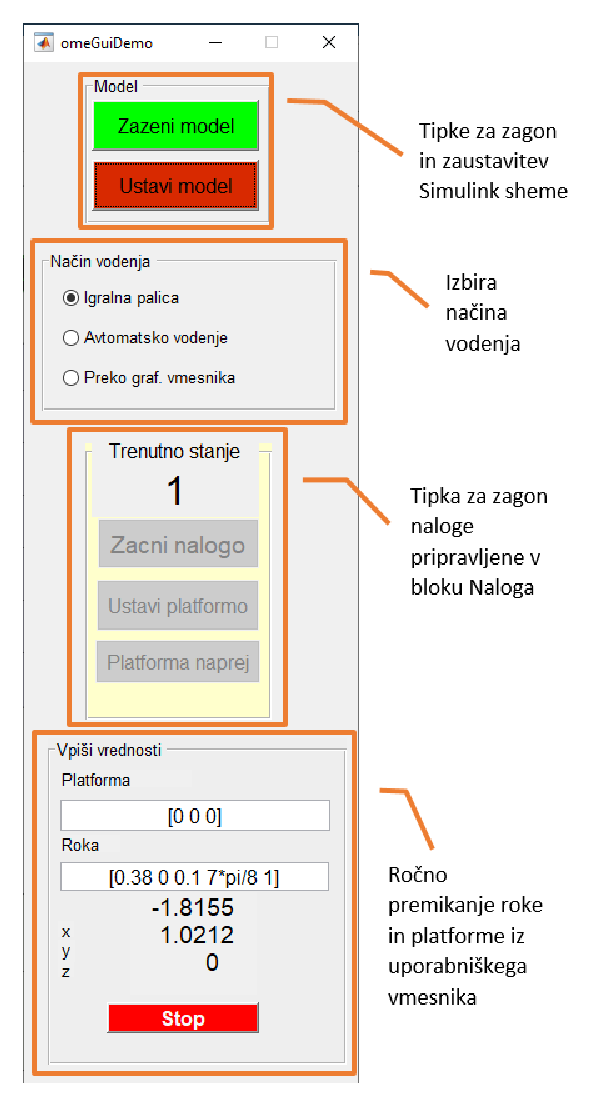
\includegraphics[draft=false]{GUI4.eps}}
	\caption{Uporabniški vmesnik za vodenje platforme.}
	\label{fig:GUI}
\end{figure}

\begin{figure}[h]
	\centering \resizebox{16cm}{!}{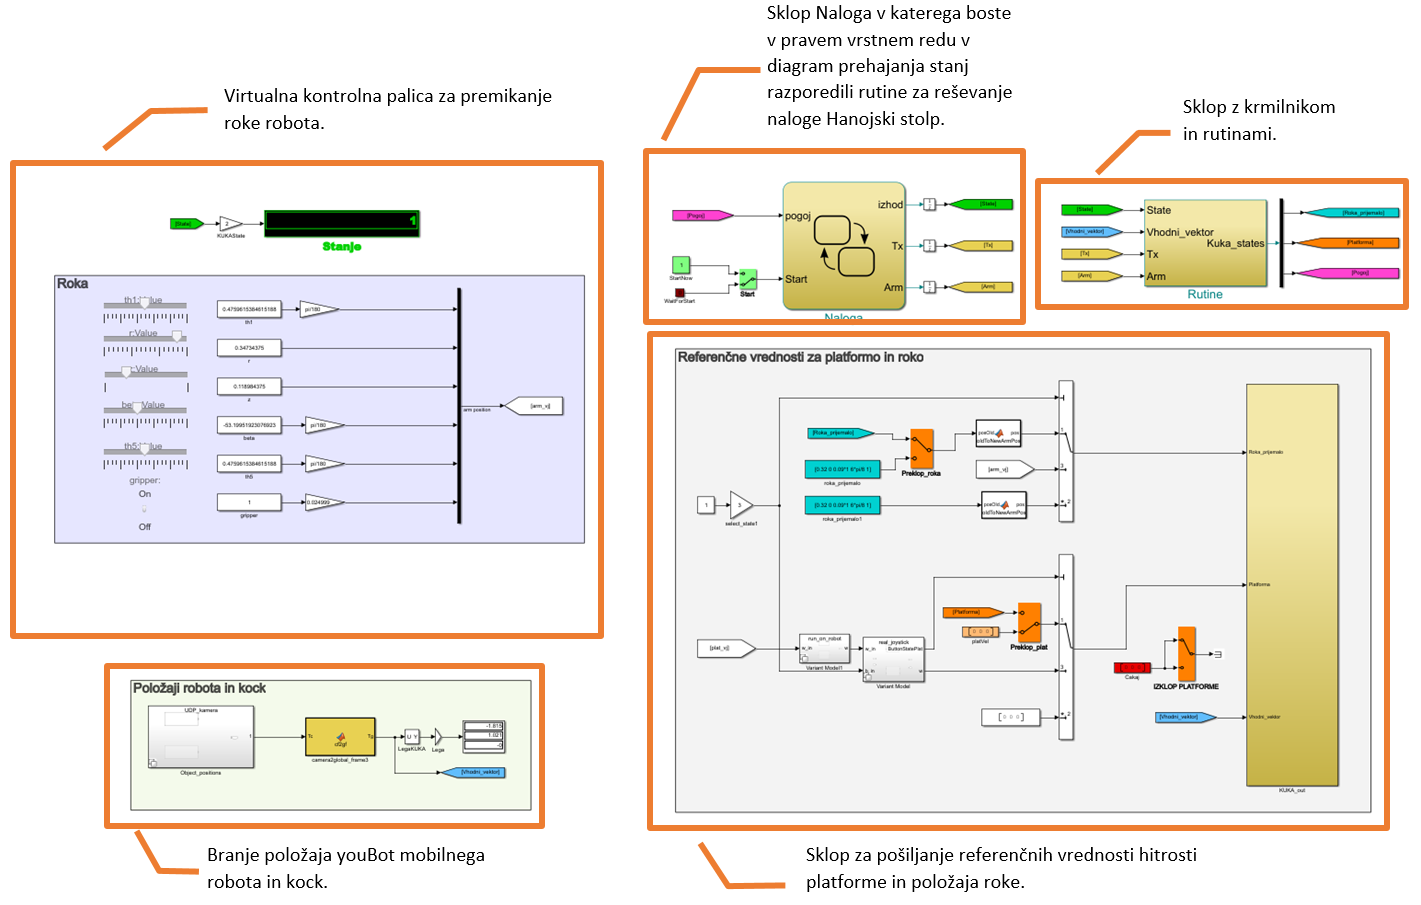
\includegraphics[draft=false]{simulink_shema4.eps}}
	\caption{Simulink model za vodenje platforme.}
	\label{fig:model}
\end{figure}

Simulnik shema, ki jo boste urejali se odpre z zagonom matlab skripte \verb|initall|. Del sheme je že vnaprej pripravljenen, v njej so z rumeno barvo označeni bloki, ki jih boste med vajo dopolnili glede na navodila v nadaljevanju skripte.

\subsection{Uporabniški vmesnik}

Uporabniški vmesnik na sliki \ref{fig:GUI} je razdeljen na več sklopov.

V sklopu \verb"Model" se nahajata gumba za zaganjanje in ustavljanje simulink  modela.
\begin{itemize}
\item Gumb \verb"Zazeni model". S pomočjo tega gumba zaženete simulink model za vodenje KUKA platforme. Ko zaženete simulink model, KUKA platforma miruje in čaka, da zaženete nalogo.
\item Gumb \verb"Ustavi model". S tem gumbom ustaviti izvajanje simulink modela.
\end{itemize}

V sklopu \verb"Način vodenja" se nahaja izbira načina vodenja mobilne platforme.
\begin{itemize}
	\item \verb"Igralna palica". Premikanje mobilne platforme s pomočjo igralne palice.
	\item \verb"Avtomatsko vodenje". Premikanje mobilne platforme preko sprogramiranega krmilnika. Zaznavanje položaja mobilne platforme poteka preko kamere na stropu. Avtomatizirano vodenje pripravite v bloku \verb|Naloga| (opisan v naslednjem poglavju).
	\item \verb"Preko graf. vmesnika". Premikanje mobilne platforme in roke preko vpisovanja željenih vrednosti hitrosti gibanja platforme in položaja roke. Vrednosti vpisujete v sklopu \verb"Vpiši vrednosti", ki je del uporabniškega vmesnika.
\end{itemize}


Sklop \verb"Trenutno stanje"
\begin{itemize}
\item Prikaz \verb"Trenutno stanje". Naloga, ki jo boste sprogramirali, je sestavljena iz posameznih podnalog, kot recimo \textit{poberi zeleno kocko}, \textit{pojdi na točko $T$}, \textit{poberi rumene kocke in jih postavi na končno mesto}, itd. Vsaka od teh podnalog ima svojo kodo, ki se izpisuje na tem mestu.
\item Gumb \verb"Zacni nalogo". Začne se izvajata sprogramirana naloga.
\item Gumb \verb"Ustavi platformo". Ta gumb izberete, ko želite začasno ustavi platformo ali izvajanje naloge. Ob kliku na gumb se referenčna hitrost za platformo postavi na vrednsot $[v_x,v_y,\omega]=[0,0,0]$. Mobilna platforma se zato ustavi, sama naloga pa še vedno teče. V primeru, da je naloga v podnalogi pobiranje kock z robotsko roko, bo roka kocke pobrala, vendar se platforma ne bo pomaknila naprej.
\item Gumb \verb"Platforma naprej". Ob kliku na gumb se referenčna hitrost za platformo postavi na vrednsot iz krmilnika za vodenje mobilne platforme in platforma se bo gibala naprej.
\end{itemize}

Sklop \verb"Vpiši vrednosti" omogoča pomikanje platforme in roke iz uporabniškega vmesnika. 

\begin{itemize}
	\item Polje \verb|Platforma|: vpišete vrednosti hitrosti za premikanje platforme. Vpišete vektor vrednosti za vodenje po osi x, osi y in rotaciji okoli osi z.
	\item Polje \verb|Roka|: vpište 5 vrednosti za postavitev roke v izbrano točko. Prve tri vrednsoti predstavljajo položaj x,y,z vrha roke, 4. vrednost je zasuk prijemala, 5. vrednost pa je vrednosti 0 za odprto prijemalo in vrednost1 za zaprto prijemalo.
	\item Prikaz položaja platforme: položaj x in y, ter rotacija platforme okoli osi z.
\end{itemize}


\newpage

\subsection{Simulink shema za vodenje platforme}

Slika \ref{fig:model} prikazuje simulink model za vodenje platforme. Glavni elementi sheme so označeni in opisani na sliki. Sklop Roka omogoča premikanje položaja robotske roke s pomočjo drsnikov.

V simulink shemi modela je najpomembnejši blok \verb"Naloga" v katerem je zapisano zaporedje ukazov, ki jih bo izvajala KUKA. S klikom na blok se odpre okno \verb"Stateflow (chart)". \verb"Stateflow (chart)" je okno za urejanje diagrama prehajanja stanj. Vsako stanje predstavlja svojo podnalogo v katero vstopite oziroma izstopite, ko je za to izpolnjen pogoj. Pogoj je izpolnjen, ko je končana posamezna podnaloga. Vsaka podnaloga ima svojo kodo, ki predstavlja stanje v katerem je celotna naloga. Seznam podnalog s kodami nalog in kodami, ko je podnaloga končana, je v tabeli \ref{tab:kodenalog}. Slika \ref{fig:stateflow1} prikazuje primer diagrama prehajanja stanj. Vsak stanje je predstavljeno z blokom, ki ima ime, vsebino in izstopni pogoj. Vsak diagram stanj, ki ga boste programirali, bo imel začetni blok \verb"Init", v katerem se bo program zadrževal, dokler ne boste v uporabniškem vmesniku kliknili na gumb \verb"Zazeni nalogo". Takrat bo izpolnjen pogoj \verb"[Start==1]" in diagram se bo prestavil v naslednje stanje. V diagramu na sliki \ref{fig:stateflow1} je to stanje z imenom \verb"Prestavi_zeleno_na_T1" in vsebino \verb"en:izhod=24;". Izvedla se bo torej rutina pobiranje zelene kocke z začetne lokacije in prestavljanja na točko $T_1$. Izstopni pogoj bloka \verb"[pogoj==124]" bo izpolnjen, ko bo KUKA prestavila zeleno kocko na točko $T_1$. Naloga se bo takrat nadaljevala z rutino s kodo \verb"25". Zadnji blok v diagramu bo blok z imenom \verb"Konec", v katerem bo ostal diagram in celotno vodenje platforme, dokler ne ugasnete simulink model.

\begin{figure}[h]
%\psfrag{x1}[][l][2.0][0]{$x_C$}
%\psfrag{y1}[][l][2.0][0]{$y_C$}
%\psfrag{z1}[][l][2.0][0]{$z_C$}
%\psfrag{x3}[][l][2.0][0]{$x_K$}
%\psfrag{y3}[][l][2.0][0]{$y_K$}
%\psfrag{z3}[][l][2.0][0]{$z_K$}
\centering \resizebox{10cm}{!}{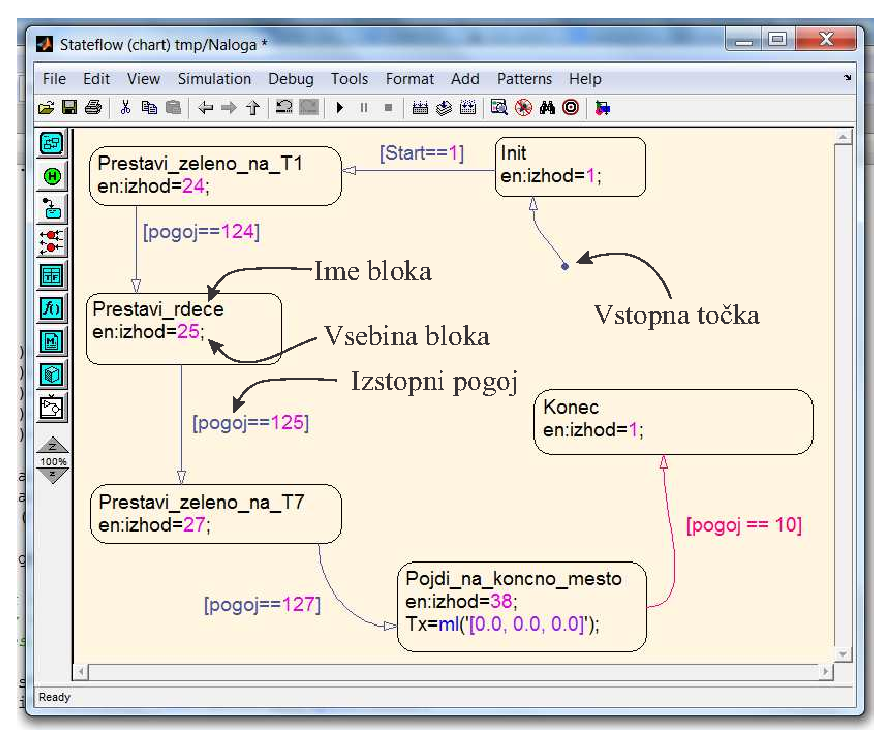
\includegraphics[draft=false]{stateflow.eps}}
\caption{Diagram prehajanja stanj za primer preproste naloge prestavljanja zelene in rdečih kock.}
\label{fig:stateflow1}
\end{figure}

Drugi pomemben blok v simulink modelu je blok \verb"Rutine" v katerih se nahajajo bloki za vodenje platforme, ki se jih kliče iz diagrama prehajanja stanj. Bloki vsebujejo zaporedje referenc za robotsko roko in prijemalo, ter krmilnik za vodenje mobilne platforme.

\newpage

% Table generated by Excel2LaTeX from sheet 'Sheet1'
\begin{table}[htbp]
  \centering
  \caption{Seznam podnalog s kodami nalog in kodami, da je podnaloga končana.}
    \begin{tabular}{rrr}
    \toprule
          & Koda  & Pogoj izpolnjen \\
    \midrule
    Konec & 1     & N/A \\ \hline
    Primi kocko & 2     & 12 \\ \hline
    Odlozi kocko & 3     & 13 \\ \hline
    Pojdi do zelene (Z1) & 4     & 10 \\ \hline
    Pojdi do rdeče 1 (Rd1) & 5     & 10 \\ \hline
    Pojdi do rdeče 2 (Rd2) & 6     & 10 \\ \hline
    Pojdi do rumene 1 (Ru1) & 7     & 10 \\ \hline
    Pojdi do rumene 2 (Ru2) & 8     & 10 \\ \hline
    Pojdi do rumene 3 (Ru3) & 9     & 10 \\ \hline
    Pojdi na točko T10 & 10    & 10 \\ \hline
    Pojdi na točko T1 & 11    & 10 \\ \hline
    Pojdi na točko T2 & 12    & 10 \\ \hline
    Pojdi na točko T3 & 13    & 10 \\ \hline
    Pojdi na točko T4 & 14    & 10 \\ \hline
    Pojdi na točko T5 & 15    & 10 \\ \hline
    Pojdi na točko T6 & 16    & 10 \\ \hline
    Pojdi na točko T7 & 17    & 10 \\ \hline
    Pojdi na točko T8 & 18    & 10 \\ \hline
    Pojdi na točko T9 & 19    & 10 \\ \hline
    Primi in odloži kocko na platformo desno & 20    & 120 \\ \hline
    Odloži kocko s platforme desno & 21    & 121 \\ \hline
    Primi in odloži kocko na platformo levo & 22    & 122 \\ \hline
    Odloži kocko s platforme levo & 23    & 123 \\ \hline
    Pojdi po zeleno na Z1 in jo odloži na T1 & 24    & 124 \\ \hline
    Pojdi po rdeči kocki in ju odloži na točki T2 in T3 & 25    & 125 \\ \hline
    Pojdi po kocko na T1 in jo odloži na T4 & 26    & 126 \\ \hline
    Pojdi po kocko na T4 in jo odloži na T7 & 27    & 127 \\ \hline
    Pojdi po kocko na T7 in jo odloži na T10 & 28    & 128 \\ \hline
    Pojdi po kocki na T2 in T3 in ju odloži na T8 in T9 & 29    & 129 \\ \hline
    Miruj & 31    & 131 \\ \hline
    Pojdi po rumene kocke in jih odloži na T6, T1, T5 & 32    & 132 \\ \hline
    Odpri prijemalo & 35    & 135 \\ \hline
    Zapri prijemalo & 36    & 136 \\ \hline
    Postavi roko v lego Arm & 37    & 137 \\ \hline
    Premakni platformo na točko Tx & 38    & 10 \\
    \bottomrule
    \end{tabular}%
  \label{tab:kodenalog}%
\end{table}%
%
\newpage


%\section{Zaganjanje polne simulacije}
%
%Pri polni simulaciji se uporablja algoritme za obdelavo slike, pri čemer se ne uporablja posameznih sličic iz kamere, temveč se sličice zajema iz vizualizacije. Poleg dinamike in kinematike KUKA platforme je tako simulirana tudi kamera. Vrstni red zaganjanja posameznih programov pri polni simulaciji je naslednji.
%
%\begin{enumerate}
%\item Odprli bomo dva samostojna Matlab procesa (dva samostojna programa), tako da bomo odprli najprej en Matlab, nato pa še enega. Ker imajo vsi sodobni osebni računalniki procesorje z več jedri pomeni, da bo vsak od Matlab programov tekel na svojem procesorju in se med seboj ne bosta motila.
%\begin{enumerate}
%\item Odpri Matlab 2011b. Pojdi v direktorij kjer se nahaja simulink model vodenja KUKA platforme \newline (\verb"D:\Kapela\workWin\PedagoskoDelo\1213\PolSola\KUKA\KUKA_1").
%\item Odpri še eno dodatno okno Matlab 2011b. Pojdi v direktorij kjer se nahaja skripta za obdelavo slike \newline (\verb"D:\Kapela\workWin\PedagoskoDelo\1213\PolSola\KUKA\KUKA_1").
%\end{enumerate}
%
%\item V prvem Matlab oknu z ukazom \verb"initall" zaženete uporabniški vmesnik in shemo vodenja. V sklopu \verb"Izvajanje" izberete možnost \verb"Polna Simulacija". Model zaženete z pritskom na gumb \verb"Zazeni model".
%
%\item Na namizju poišči program \texttt{KUKA vis} in ga zaženi. Ko se bo na zaslonu prikazala vizualizacija, poišči na namizju program \texttt{Screen Capture} in ga zaženi. Program ima samo eno gumb \texttt{Start Screenshot} s katerim se zažene zajemanje slike iz vizualizacije. Ko program teče se bo nad gumbom izpisovalo število zajetih sličic na sekundo.
%
%\item \textbf{POZOR!} Program za zajemanje slike iz vizualizacije deluje tako, da zajema slike zaslona na območju kjer teče program vizualizacije. To je podobno kot, če bi za vsako od sličic pritisnili na tipkovnici tipko \texttt{Print screen}. \textbf{Program vizualizacije mora zato vedno ostati na istem mestu in nič ga ne sme prekriti.} Zato bo potrebno velikost oken Matlaba zmanjšati, da ne bosta prekrili okna vizualizacije.
%
%%\item Pojdite do drugega programa Matlab. \textbf{Okno Matlab programa zmanjšajte, tako da ne prekriva okna vizualizacije.} Odprete skripto \texttt{KUKA_SimKamera.m} in jo zaženete. Ko se v ukaznem oknu Matlaba izpiše \verb"d = 1", pomeni, da so bile pozicije kock določene in takrat lahko z gumbom \verb"Zacni nalogo" zaženete nalogo, ki ste jo sprogramirali. če Matlab vrača napako je najbolje Matlab okno zapreti in odpreti novega. Običajno se lahko pri večkratnem zaganjanju skripte pojavijo težave z UDP komunikacijo med skripto in simulink modelom. Takrat je najbolje Matlab zapreti in odpreti novega.
%%
%%\item \textbf{POZOR! Zelo pomemben je tudi vrstni red zapiranja programov.} Ko je naloga bodisi uspešno ali neuspešno končana in želite poskusiti znova je vrstni red zapiranja programov sledeč.
%%
%%\begin{enumerate}
%%    \item Najprej prekinete obdelavo slike. Kliknete v ukazno okno Matlaba, kjer poteka obdelava slike. Nato na tipkovnici kliknete tipke \texttt{CTRL+C}. S tem "nasilno" prekinete izvajanje obdelave slike. Nato v ukazni vrstici zaženete ukaz \verb"killUdp".
%%    \item Nato ugasnete program \texttt{FPS Screen Capture} (ki ste zagnali z ikono \texttt{Screen Capture}).
%%    \item Nato lahko sedaj ugasnete vizualizacijo (ki ste zagnali z ikono \texttt{KUKA vis}). če ste slučajno že ustavili izvajanje simulink modela, se okno za vizualizacijo ne bo želelo zapreti. Program za vizualizacijo namreč stalno pričakuje podatke iz simulink sheme in če jih ne dobi se "obesi" (ujame oziroma "zacikla" se v zanki za branje podatkov iz simulink sheme). če se to zgodi, zaženite simulink model in vizualizacijo boste lahko zaprli. Program za vizualizacijo namreč dobi nove podatke iz sheme in zapusti zanko za branje podatkov.
%%    \item Nazadnje lahko ustavite simulink model z izbiro gumba \verb"Ustavi model".
%%\end{enumerate}
%
%\end{enumerate}




\section{Odprava napake perspektive kamere}

Kamera zaznava sceno kot projekcijo predmetov na ravnino, ki je vzporedna z lečo kamere. Ravnino lahko postavimo na poljubno oddaljenost od kamere. Relativna oddaljenost predmetov se ne bo spremenila, spremenila pa se bo njihova absolutna oddaljenost. Zato je smiselno postaviti ravnino kamere na razdalje, kjer se predmeti resnično nahajajajo. V našem primeru so to tla, ki so nahajajo na oddaljenosti $2.81$ metra od kamere. Ker z-os koordinatnega sistema kamere kaže navzdol (glej sliko \ref{fig:AllFrames}), je torej z koordinata ravnine tal na $z=-2.81$ $m$. Seveda pa predmeti niso ploščati, vsak predmet ima tudi svojo višino. Ker zaznavamo značilnosti in barve kock, ki se nahajajo na zgornji ploskvi, pride do napake perspektive, saj kot rečeno, predmeti niso ploščati, in so njihove zgornje ploskve bližje kameri kot projekcijska ravnina, ki smo jo postavili na oddaljenost 2.81 metra od kamere. Napaka perspektive se veča z razliko med projekcijsko ravnino in dejansko oddaljenosjo predmeta od kamere ter z oddaljenostjo predmeta od osi kamere. Primer prikazujeta sliki \ref{fig:PredmetiPerspektiva} in \ref{fig:NapakaPerspektive}. Slika \ref{fig:PredmetiPerspektiva} prikazuje predmete, ki so na različnih višinah in oddaljenostih od osi kamere, slika \ref{fig:NapakaPerspektive} pa prikazuje napake, ki nastanejo zaradi perspektive.

\begin{figure}[h]
\centering \resizebox{10cm}{!}{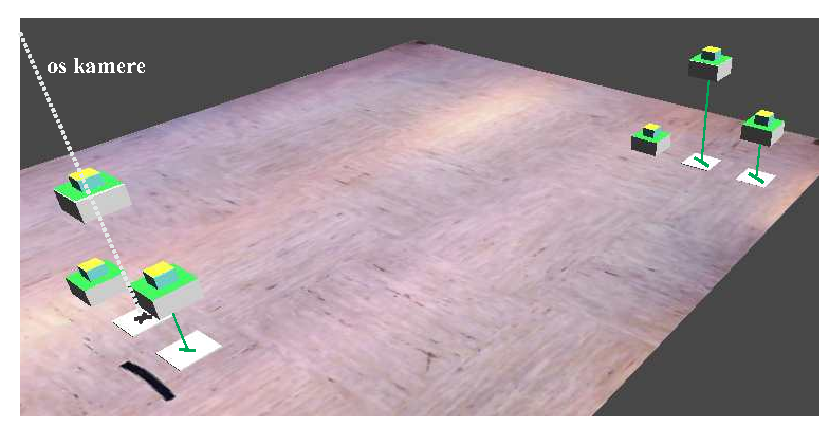
\includegraphics[draft=false]{perspektiva-2.eps}}
\caption{Predmeti v sceni, ki jo vidi kamera, se nahajajo na različnih višinah. To privede do napake določanja pozicije teh objektov, ki so prikazane na spodnji sliki.}
\label{fig:PredmetiPerspektiva}
\end{figure}

\begin{figure}[h]
\centering \resizebox{10cm}{!}{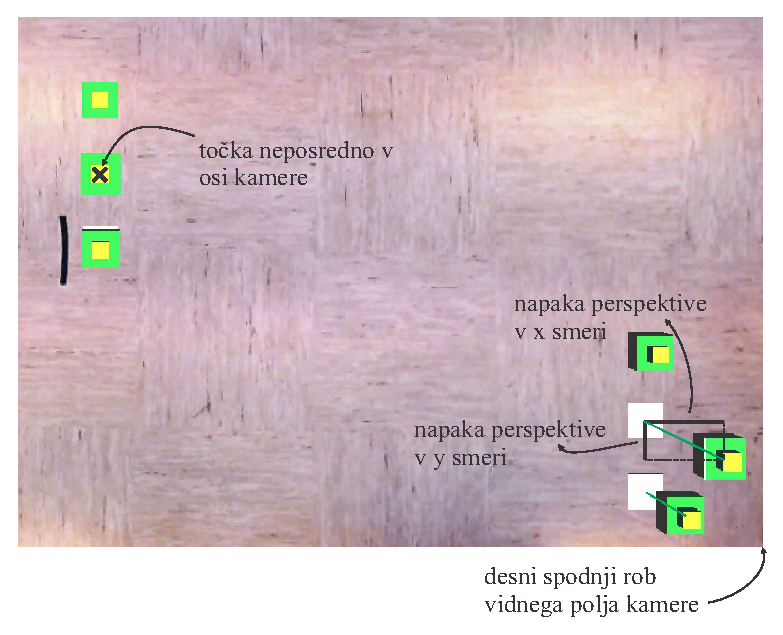
\includegraphics[draft=false]{perspektiva-1.eps}}
\caption{Prikaz napake pozicij zaradi perspektive.}
\label{fig:NapakaPerspektive}
\end{figure}

Program za določanje lege predmetov torej zaradi napake perspektive vrne pozicijo predmeta, ki ni točna. Jo je pa mogoče zlahka odpraviti, če poznamo višino zgornje ploskve predmeta. Napako je enostavno odpraviti s homogeno transformacijsko matriko enačbe leče.


\begin{figure}[ht]
\centering
\begin{minipage}[b]{0.35\linewidth}
\centering
\psfrag{G}[][l][2.0][0]{$G$}
\psfrag{C}[][l][2.0][0]{$C$}
\psfrag{O}[][l][2.0][0]{$O$}
\psfrag{pc}[][r][2.0][0]{$\prescript{C}{}p_K$}
\psfrag{p}[][l][2.0][0]{$\prescript{G}{}p_K$}
\psfrag{Hg}[][l][2.0][0]{$\prescript{C}{}H_G$}
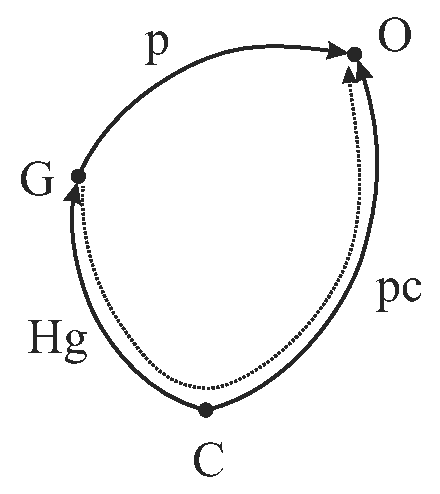
\includegraphics[width=\textwidth]{KS1-1.eps}
\caption{Podana lega globalnega koordinatnega sistema glede na koordinatni sistem kamere. Transformacijska matrika je $\prescript{C}{}H_G$.}
\label{fig:TransfKamGlob}
\end{minipage}
\hspace{1.5cm}
\begin{minipage}[b]{0.35\linewidth}
\centering
\psfrag{G}[][l][2.0][0]{$G$}
\psfrag{C}[][l][2.0][0]{$C$}
\psfrag{O}[][l][2.0][0]{$O$}
\psfrag{pc}[][r][2.0][0]{$\prescript{C}{}p_K$}
\psfrag{p}[][l][2.0][0]{$\prescript{G}{}p_K$}
\psfrag{Hc}[][C][2.0][0]{$\prescript{G}{}H_C$}
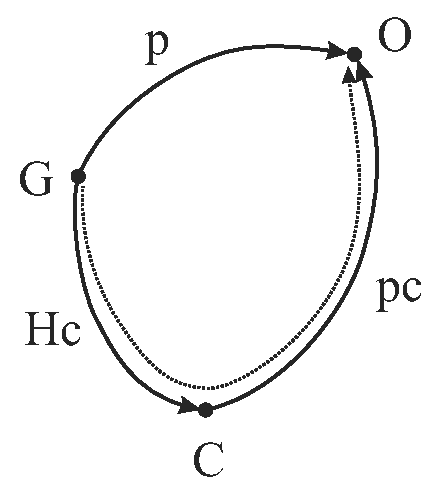
\includegraphics[width=\textwidth]{KS1-2.eps}
\caption{Podana lega koordinatnega sistema kamere glede na globalni koordinatni sistem. Transformacijska matrika je $\prescript{G}{}H_C$.}
\label{fig:TransfGlobKam}
\end{minipage}
\end{figure}

\subsection{Transformacija iz koordinatnega sistema kamere v globalni koordinatni sistem}
Prvi korak je, da postavimo nov koordniatni sistem v os kamere. To bo naš novi globalni koordinatni sistem. Da določimo lego KUKA platforme v globalnem koordinatnem sistemu, je potrebno lego platforme iz koordinatnega sistema kamere transformirati v globalni koordinatni sistem s pomočjo transformacije, ki opisuje medsebojno lego koordinatnega sistema kamere in globalnega koordinatnega sistema. Lega platforme je določena s pozicijo platforme $p_K = [x_K, y_K]$, ter orientacijo, ki jo določa kot $\varphi$ okoli vertikalne z osi. Najprej določimo pozicijo v globalnem koordinatnem sistemu $\prescript{G}{}p_K$. Robotski vid nam vrača pozicijo platforme $\prescript{C}{}p_K$ v koordinatnem sistemu kamere. Slika \ref{fig:TransfGlobKam} podaja diagram transformacij za določitev pozicije platforme v globalnem koordinatnem sistemu.

\begin{equation}
    \prescript{G}{}p_K = \prescript{G}{}H_C \, \cdot \prescript{C}{}p_K.
\end{equation}

Potrebno je torej določiti transformacijo $\prescript{G}{}H_C$, ki podaja lego koordinatnega sistema kamere v globalnem koordinatnem sistemu. Slika \ref{fig:TransfKamGlob} prikazuje, da je mogoče izračunati $\prescript{C}{}p_K$ tudi, če poznamo lego globalnega koordinatnega sistema glede na koordinatni sistem kamere $\prescript{G}{}H_C$. Takrat velja

\begin{equation}
    \prescript{G}{}p_K = \prescript{C}{}H_G^{-1} \, \cdot \prescript{C}{}p_K,
\end{equation}

saj je

\begin{equation}
\prescript{C}{}H_K^{-1} = \prescript{G}{}H_C.
\end{equation}

Pozicijo v globalnem koordinatnem sistemu $\prescript{G}{}p_K$ torej lahko določimo na dva načina:

\begin{itemize}
\item Podamo lego globalnega koordinatnega sistema glede na koordinatni sistem kamere. Transformacijsko matriko označimo kot $\prescript{C}{}H_G$.
\item Podamo lego koordinatnega sistema kamere glede na globalni koordinatni sistem. Transformacijsko matriko označimo kot $\prescript{G}{}H_C$.
\end{itemize}

Orientacijo platforme določa kot $\varphi$, ki podaja kot zasuka okoli z-osi od x-osi. Ko je x-os koordinatnega sistema, ki se nahaja na platformi, poravnan z x-osjo koordinatnega sistema kamere je kot $\varphi$ enak nič. če je x-os koordinatnega sistema platforme zavrtena v pozitivni smeri okoli z-osi globalnega koordinatnega sistema, ki kaže navzgor, je kot $\varphi$ večji od nič.

Os x globalnega koordinatnega sistema in koordinatnega sistema kamere sta poravnana, z-os globalnega koordinatnega sistema pa kaže v nasprotno smer kot z-os koordinatnega sistema kamere. Kot $\prescript{G}{}\varphi$ v globalnem koordinatnem sistemu je zato

\begin{equation}
    \prescript{G}{}\varphi = - \prescript{C}{}\varphi.
\end{equation}

Spremeni se torej le predznak kota $\varphi$.


\subsection{Perspektivična transformacija}

Napako perspektive je mogoče odpraviti s pomočjo perspektivične transformacijske matrike $H_f$

\begin{equation}
H_f = w \,
\begin{bmatrix}
1 & 0 & 0 & 0 \cr
0 & 1 & 0 & 0 \cr
0 & 0 & 1 & 0 \cr
0 & 0 & -\frac{1}{f} & 1
\end{bmatrix}.
\end{equation}

V teoriji perspektivične transformacije $f$ predstavlja žariščno razdaljo leče, ki preslikava predmet. V našem primeru ta vrednost ni povezana z goriščno razdaljo kamere, ki se uporablja za robotski vid, temveč je vrednost $f$ povezana z razmerjem višine predmetov in višino kamere za robotski vid. Zanima nas namreč projekcija markerjev objektov na ravnino tal in ne na slikovni senzor kamere. Vrednost $f$ je torej različna za vsak predmet, saj je odvisna od njegove višine oziroma od oddaljenosti markerja objekta od tal. Vrednost $f$ bo torej potrebno izračunati. Zapišimo torej naslednjo matrično enačbo:

\begin{equation}
w \,
\begin{bmatrix}
1 & 0 & 0 & 0 \cr
0 & 1 & 0 & 0 \cr
0 & 0 & 1 & 0 \cr
0 & 0 & -\frac{1}{f} & 1
\end{bmatrix}
\left[
\begin{array}{c}
x^p_K \\
y^p_K \\
z^p_K \\
1
\end{array}
\right]
=
\left[
\begin{array}{c}
x_K \\
y_K \\
z_K \\
1
\end{array}
\right].
\end{equation}

iz katere dobimo štiri enačbe s štirimi naznankami:

\begin{eqnarray}
x_K = w x^p_K \\
y_K = w y^p_K \\
z_K = w z^p_K \\
w(-\frac{1}{f}z^p_K+1)=1,
\end{eqnarray}

Neznanke so koordinate prave pozicije objektov $x_K$, $y_K$, žarišče $f$ ter skalirni faktor $w$. Izračunajmo najprej skalirni faktor $w$ iz tretje enačbe, saj poznamo tako $z_K$ kot $z^p_K$. Tla so od kamere oddaljena za $h_k = 2.81m$, marker je projeciran na ravnino tal, torej je $z^p_K = h_k$. Vrednost $z_K$ je prava oddaljenost od kamere, ki je za višino objekta bližje kameri kot so tla, torej $z_K = h_k - h_O$, kjer je $h_O$ višina objekta. Faktor $w$ je torej

\begin{equation}
w = \frac{z_K}{z^p_K} = \frac{h_k - h_O}{h_k}.
\end{equation}

Iz četrte enačbe izračunajmo žarišče $f$

\begin{equation}
f =  -\frac{h_k}{h_O}(h_k-h_O).
\end{equation}


\begin{figure}[h]
\psfrag{x1}[][l][2.0][0]{$x_C$}
\psfrag{y1}[][l][2.0][0]{$y_C$}
\psfrag{z1}[][l][2.0][0]{$z_C$}
\psfrag{x2}[][l][2.0][0]{$x_G$}
\psfrag{y2}[][l][2.0][0]{$y_G$}
\psfrag{z2}[][l][2.0][0]{$z_G$}
\psfrag{dol}[][l][2.0][0]{$wi$}
\psfrag{sir}[][l][2.0][0]{$hi$}
\psfrag{x3}[][l][2.0][0]{\color{white}$x_K$}
\psfrag{y3}[][l][2.0][0]{\color{white}$y_K$}
\psfrag{z3}[][l][2.0][0]{\color{white}$z_K$}
\centering \resizebox{10cm}{!}{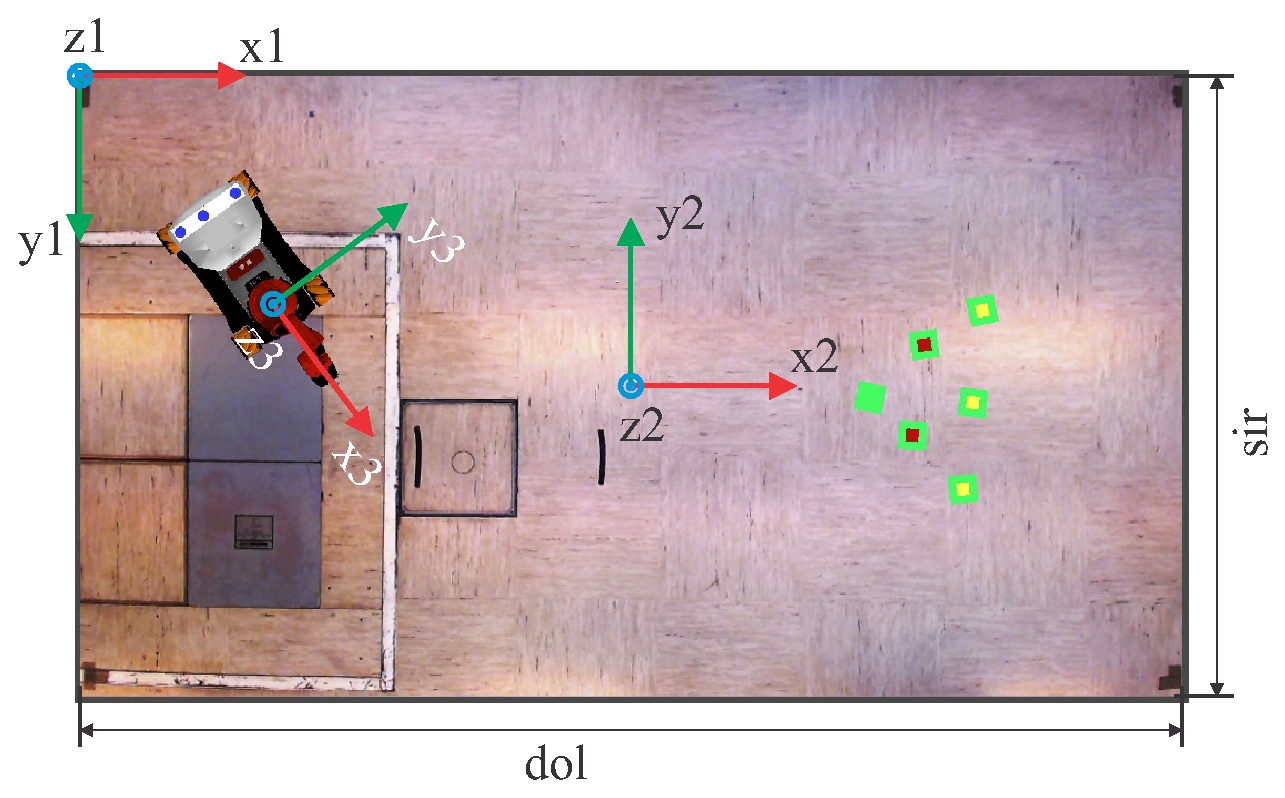
\includegraphics[draft=false]{frames-1.eps}}
\caption{Koordinatni sistem kamere, koordinatni sistem KUKE in globalni koordinatni sistem.}
\label{fig:AllFrames}
\end{figure}

V shemi modela vodenja KUKA platforme odprite blok \verb"camera2global_frame", katerem se nahaja funkcija \verb"cf2gf". Funkcija \newline \verb"function Tg = cf2gf(Tc)" pretvori koordinate iz koordinatnega sistema kamere v globalni koordinatni sistem. Vhod je vektor \verb"Tc", ki vsebuje koordinate KUKA platforme (1:3), ter koordinate 6 kock (4:6, 7:9, 10:12, 13:15, 16:18, 19:21) v koordinatnem sistemu kamere. Vsega skupaj je torej 7 objektov. Izhod je vektor \verb"Tg", v katerem so vhodne točke \verb"Tc" transformirane v globalni koordinatni sistem. Del funkcije je že pripravljen, del funkcije pa morate dopisati vi.

Vrstni red transformacij za pretvorbo iz koordinatnega sistema kamere v globalni koordinatni sistem in odprava zaradi projekcije je torej:

\begin{enumerate}
\item Zapis točke v koordinatnem sistemu kamere
\begin{itemize}
    \item $\prescript{C}{}p$ ... točka v koordinatnem sistemu kamere
    \item $x_c,\,\, y_c$ ... $x$ in $y$ koordinate v koordinatnem sistemu kamere
\end{itemize}

\begin{equation}
\prescript{C}{}p =
\left[
\begin{array}{c}
x_c \\
y_c \\
-h_k \\
1
\end{array}
\right]
\end{equation}

\item Pretvorba iz koordinatnega sistema kamere v globalni koordinatni sistem
\begin{itemize}
    \item $\prescript{G}{}H_C$ ... homogena transformacijska matrika, ki podaja lego koordinatnega sistema kamere glede na globalni koordinatni sistem.
    \item $\prescript{G,p}{}p$ ... točka v globalnem koordinatnem sistemu, pred odpravo napake projekcije na tla.
\end{itemize}

\begin{equation}
    \prescript{G,p}{}p = \prescript{G}{}H_C \cdot \, \prescript{C}{}p
\end{equation}

\item Odprava napake zaradi projekcije
\begin{itemize}
    \item $\prescript{G}{}p$ ... točka v globalnem koordinatnem sistemu po odpravi napake projekcije
    \item $H_f$ ... perspektivična transformacijska matrika
\end{itemize}

\begin{equation}
    \prescript{G}{}p_K = H_f \cdot \, \prescript{G,p}{}p_K
\end{equation}

\item Pretvorba kota orientacije objekta iz koordinatnega sistema kamere v globalni koordinatni sistem.

\end{enumerate}

\begin{mdframed}[backgroundcolor=yellow!20, shadow=true,roundcorner=8pt]

V simulink modelu je potrebno napraviti naslednje korake:

\begin{enumerate}

\item V shemi modela vodenja KUKA platforme odprite blok \verb"camera2global_frame", katerem se nahaja funkcija \verb"cf2gf". Funkcija \newline \verb"function Tg = cf2gf(Tc)" pretvori koordinate iz koordinatnega sistema kamere v globalni koordinatni sistem. Vhod je vektor \verb"Tc", ki vsebuje koordinate KUKA platforme \verb"(1:3)", ter koordinate 6 kock (\verb"(4:6)", \verb"(7:9)", \verb"(10:12)", \verb"(13:15)", \verb"(16:18)", \verb"(19:21)") v koordinatnem sistemu kamere. Vsega skupaj je torej 7 objektov. Izhod je vektor \verb"Tg", v katerem so vhodne točke \verb"Tc" transformirane v globalni koordinatni sistem. Del funkcije je že pripravljen, del funkcije pa morate dopisati vi.

\item Kodo boste vpisovali med komentarja
\\ %
\\ %
\small %
\textcolor[rgb]{0.50,0.50,0.50}{\texttt{$\%\%\%\%\%\%\%\%\%\%\%\%\%\%\%\%\%\%\%\%\%\%\%\%\%\%\%\%\%\%\%\%$ }} \\%
\textcolor[rgb]{0.50,0.50,0.50}{\texttt{$\%$  TUKAJ PISEJO STUDENTI}} \\%
\textcolor[rgb]{0.50,0.50,0.50}{\texttt{$\%\%\%\%\%\%\%\%\%\%\%\%\%\%\%\%\%\%\%\%\%\%\%\%\%\%\%\%\%\%\%\%$ }} \\%
in
\\
\textcolor[rgb]{0.50,0.50,0.50}{\texttt{$\%\%\%\%\%\%\%\%\%\%\%\%\%\%\%\%\%\%\%\%\%\%\%\%\%\%\%\%\%\%\%\%$ }} \\%
\textcolor[rgb]{0.50,0.50,0.50}{\texttt{$\%$  DO TUKAJ PISEJO STUDENTI}} \\%
\textcolor[rgb]{0.50,0.50,0.50}{\texttt{$\%\%\%\%\%\%\%\%\%\%\%\%\%\%\%\%\%\%\%\%\%\%\%\%\%\%\%\%\%\%\%\%$ }}
\normalsize %
\item Zapis matrike za transformacijo v globalni koordinatni sistem
\\
\small %
\textcolor[rgb]{0.50,0.50,0.50}{\texttt{$\%$  Nadomestite znake \emph{\#} v spodnji matriki z ustreznimi vrednostimi}} \\%
\texttt{\tab{H = [} \tab{\emph{\#}  \emph{\#}  \emph{\#}  \emph{\#}; ...}} \\
\texttt{\tab{} \tab{\emph{\#}  \emph{\#}  \emph{\#}  \emph{\#}; ...}} \\
\texttt{\tab{} \tab{\emph{\#}  \emph{\#}  \emph{\#}  \emph{\#}; ...}} \\
\texttt{\tab{} \tab{\emph{\#}  \emph{\#}  \emph{\#}  \emph{\#}];}}
%\texttt{\tab{H = [} \tab{1  0  0  wi/2; ...}} \\
%\texttt{\tab{} \tab{0 -1  0  hi/2; ...}} \\
%\texttt{\tab{} \tab{0  0 -1  0; ...}} \\
%\texttt{\tab{} \tab{0  0  0  1];}} \\
%\texttt{    H = [1  0  0  wi/2; ...} \\
%\texttt{         0 -1  0  hi/2; ...} \\
%\texttt{         0  0 -1  0; ...} \\
%\texttt{         0  0  0  1];}
\normalsize %
\item Zapis vektorja pozicije objekta v koordinatnem sistemu kamere
\\ %
\small %
\texttt{    pc = [xc; yc; -vk; 1];}
\normalsize %
\item Transformacija pozicije iz koordinatnega sistema kamere v globalni koordinatni sistem
\\ %
\small %
\texttt{    pp = \emph{ZAPIŠI USTREZNO TRANSFORMACIJO};}
\normalsize %
\item Izračun parametrov perspektivične transformacije
\\ %
\small %
\textcolor[rgb]{0.50,0.50,0.50}{\texttt{$\%$  Izračunaj f in w parametra}} \\%
\textcolor[rgb]{0.50,0.50,0.50}{\texttt{$\%$  hc ... višina kamere}} \\%
\textcolor[rgb]{0.50,0.50,0.50}{\texttt{$\%$  ho ... višina objekta}} \\%
\texttt{    f = \emph{ZAPIŠI USTREZNI IZRAZ};} \\
\texttt{    w = \emph{ZAPIŠI USTREZNI IZRAZ};}
\normalsize %
\item Transformacijska matrika perspektivične transformacije
\\ %
\small %
\textcolor[rgb]{0.50,0.50,0.50}{\texttt{$\%$  Nadomestite znake \emph{\#} v spodnji matriki z ustreznimi vrednostimi}} \\%
\texttt{\tab{Hf = } \tab{w*[} \tab{\emph{\#}  \emph{\#}  \emph{\#}  \emph{\#}; ...}} \\
\texttt{\tab{} \tab{} \tab{\emph{\#}  \emph{\#}  \emph{\#}  \emph{\#}; ...}} \\
\texttt{\tab{} \tab{} \tab{\emph{\#}  \emph{\#}  \emph{\#}  \emph{\#}; ...}} \\
\texttt{\tab{} \tab{} \tab{\emph{\#}  \emph{\#}  \emph{\#}  \emph{\#}];}}
\normalsize %
\item Izračun pozicije objekta v globalnem koordinatnem sistemu z odpravljeno napako perspektive
\\ %
\small %
\texttt{    pg = Hf*pp;}
\normalsize %
\item Zapis pozicije in orientacije objekta v globalnem koordinatnem sistemu
\\ %
\small %
\texttt{    xo = pg(1);} \\
\texttt{    yo = pg(2);} \\
\texttt{    fio = -fic;}
\normalsize %
\item Zapis v funkciji med komentarji je torej
%\begin{tabular}
\\ %
\small %
\textcolor[rgb]{0.50,0.50,0.50}{\texttt{$\%\%\%\%\%\%\%\%\%\%\%\%\%\%\%\%\%\%\%\%\%\%\%\%\%\%\%\%\%\%\%\%$ }} \\%
\textcolor[rgb]{0.50,0.50,0.50}{\texttt{$\%$  TUKAJ PISEJO STUDENTI}} \\%
\textcolor[rgb]{0.50,0.50,0.50}{\texttt{$\%\%\%\%\%\%\%\%\%\%\%\%\%\%\%\%\%\%\%\%\%\%\%\%\%\%\%\%\%\%\%\%$ }} \\%
\textcolor[rgb]{0.50,0.50,0.50}{\texttt{$\%$  Nadomestite znake \emph{\#} v spodnji matriki z ustreznimi vrednostimi}} \\%
\texttt{\tab{H = [} \tab{\emph{\#}  \emph{\#}  \emph{\#}  \emph{\#}; ...}} \\
\texttt{\tab{} \tab{\emph{\#}  \emph{\#}  \emph{\#}  \emph{\#}; ...}} \\
\texttt{\tab{} \tab{\emph{\#}  \emph{\#}  \emph{\#}  \emph{\#}; ...}} \\
\texttt{\tab{} \tab{\emph{\#}  \emph{\#}  \emph{\#}  \emph{\#}];}} \\
\texttt{    pc = [xc; yc; -vk; 1];} \\
\texttt{    pp = \emph{ZAPIŠI USTREZNO TRANSFORMACIJO};}\\
\textcolor[rgb]{0.50,0.50,0.50}{\texttt{$\%$  Izračunaj f in w parametra}} \\%
\textcolor[rgb]{0.50,0.50,0.50}{\texttt{$\%$  hc ... višina kamere}} \\%
\textcolor[rgb]{0.50,0.50,0.50}{\texttt{$\%$  ho ... višina objekta}} \\%
\texttt{    f = \emph{ZAPIŠI USTREZNI IZRAZ};} \\
\texttt{    w = \emph{ZAPIŠI USTREZNI IZRAZ};}\\
\textcolor[rgb]{0.50,0.50,0.50}{\texttt{$\%$  Nadomestite znake \emph{\#} v spodnji matriki z ustreznimi vrednostimi}} \\%
\texttt{\tab{Hf = [} \tab{\emph{\#}  \emph{\#}  \emph{\#}  \emph{\#}; ...}} \\
\texttt{\tab{} \tab{\emph{\#}  \emph{\#}  \emph{\#}  \emph{\#}; ...}} \\
\texttt{\tab{} \tab{\emph{\#}  \emph{\#}  \emph{\#}  \emph{\#}; ...}} \\
\texttt{\tab{} \tab{\emph{\#}  \emph{\#}  \emph{\#}  \emph{\#}];}}\\
\texttt{    pg = w*Hf*pp;} \\
\texttt{    xo = pg(1);} \\
\texttt{    yo = pg(2);} \\
\texttt{    fio = -fic;} \\
\textcolor[rgb]{0.50,0.50,0.50}{\texttt{$\%\%\%\%\%\%\%\%\%\%\%\%\%\%\%\%\%\%\%\%\%\%\%\%\%\%\%\%\%\%\%\%$ }} \\%
\textcolor[rgb]{0.50,0.50,0.50}{\texttt{$\%$  DO TUKAJ PISEJO STUDENTI}} \\%
\textcolor[rgb]{0.50,0.50,0.50}{\texttt{$\%\%\%\%\%\%\%\%\%\%\%\%\%\%\%\%\%\%\%\%\%\%\%\%\%\%\%\%\%\%\%\%$ }}
\normalsize %
%\end{tabular}
\end{enumerate}

\end{mdframed}

\section{Vodenje vsesmerne platforme v globalnem in lokalnem koordinatnem sistemu}

Platformo vodimo tako, da določamo hitrost gibanja platforme v treh prostostnih stopnjah $v_K = \begin{bmatrix}
v_x \\ v_y \\ \omega_z \end{bmatrix}$:
\begin{itemize}
\item hitrost gibanja v $x$ smeri $v_x$,
\item hitrost gibanja v $y$ smeri $v_y$,
\item hitrost rotiranja okoli $z$ osu $\omega_z$.
\end{itemize}

Vodenje lahko poteka v lokalnem koordinatnem sistemu platforme ali v globalnem koordinatnem sistemu. V primeru vodenja v globalnem koordinatnem sistemu je potrebno hitrost iz globalnega koordinatnega sistem transformirati v lokalni koordinatni sistem. Hitrost v globalnem koordinatnem sistemu je potrebno za kot $\varphi$ (orientacija vsesmerne platforme) zarotirati okoli z-osi v lokalni koordinatni sistem platforme:

\begin{mdframed}[backgroundcolor=yellow!20, shadow=true,roundcorner=8pt]

\begin{equation}\label{eq:hitrosti}
    \prescript{lokalni\,\,k.s.}{}v_K = Rot_z(\varphi)^{-1}\,\cdot\prescript{globalni\,\,k.s.}{}v_K
\end{equation}

\begin{itemize}
\item $\prescript{lokalni\,\,k.s.}{}v_K$ ... hitrost v lokalnem koordinatnem sistemu KUKA platforme
\item $Rot_z(\varphi)$ ... rotacijska matrika okoli z-osi za kot $\varphi$
\item $\prescript{globalni\,\,k.s.}{}v_K$ ... hitrosti podane v globalnem koordinatnem sistemu.
\end{itemize}


\begin{enumerate}
\item Odprite blok \verb"KUKA_out/trans_w". V bloku \verb"KUKA_out" se nahaja funkcija \verb"trans_w" v bloku \verb"trans_w".
\begin{itemize}
\item Vhod v funkcijo je
\begin{itemize}
\item kot \verb"fi" ($\varphi$) orientacija vsesmerne platforme v globalnem koordinatnem sistemu,
\item ter hitrost \verb"w" ($\prescript{globalni\,\,k.s.}{}v_K$) v globalnem koordinatnem sistemu.
\end{itemize}
\item Izhod iz funkcije je hitrost \verb"w_out" ($\prescript{lokalni\,\,k.s.}{}v_K$) v lokalnem koordinatnem sistemu.
\end{itemize}
\item Vpišite enačbo za transformacijo hitrosti v globalnem koordinatnem sistemu \verb"w" v hitrost v lokalnem koordinatnem sistemu \verb"w_out" po enačbi \ref{eq:hitrosti}.
\end{enumerate}

\end{mdframed}

Ko sedaj uporabljate za premikanje oziroma vodenje platforme pravo ali virtualno igralno palico, premikanje platforme poteka v globalnem koordinatnem sisteme, medtem, ko je predtem premikanje platforme potekalo v lokalnem koordinatnem sistemu platforme. Premik po osi x bo torej pomikal platformo v smeri osi \verb|x2| (glej sliko \ref{fig:AllFrames}), ker je pomikanje sedaj izvedeno v globalnem koordinatnem sistemu, pomikanje v lokalnem koordinatnem sistemu platforme pa je bilo v smeri osi \verb|x3|.

\section{Pozicijsko vodenje KUKA platforme}

Ko poznamo pravo lego KUKA platforme v prostoru, lahko načrtamo pozicijsko vodenje mobilne platforme. Vhod v pozicijsko vodenje platforme je željena lega (pozicija in orientacija) platforme in trenutna lega platforme. Cilj je seveda krmiliti platformo tako, da se platforma pripelje v željeno lego, da bo torej napaka med željeno in dejansko lego manjša od vnaprej določene najmanjše dovoljene napake. Krmilnik za pozicijsko vodenje se nahaja v glavnem bloku \verb"Rutine" v podbloku \newline \verb"Rutine/Pojdi_do_Tocke/Pojdi_na_T/Krmilnik". Vhod v blok \verb"Krmilnik" sta
\begin{itemize}
\item \verb"P_robot" - trenutna lega platforme v globalnem koordinatnem sistemu in
\item \verb"Ciljna tocka" - željena lega platforme v globalnem koordinatnem sistemu.
\end{itemize}

Izhod iz bloka sta
\begin{itemize}
\item \verb"Platforma" - željena hitrost gibanja platforme $[v_x,v_y,\omega]$ v globalnem koordinatnem sistemu in
\item \verb"Na poziciji" - pogoj, ki signalizira, da je platforma dosegla željeno lego. Pogoj je izpolnjen, ko je napaka med željeno in dejansko lego dovolj majhna.
\end{itemize}

Krmilnik, ki je potreben za uspešno vodenje platforme je lahko zelo preprost proporcionalni krmilnik (P-krmilnik):
\begin{enumerate}
\item \textbf{Izračun napake $e_r$ med željeno lego $p_t$ in dejansko lego $p_r$}
\begin{equation}
    e_r = p_t - p_r
\end{equation}
\item \textbf{Izračun željene hitrosti gibanja platforme}
\begin{enumerate}
\item Množenje napake s proporcionalnim ojačanjem K, ki je lahko začetek kar $K=[1,1,1]$.
\begin{equation}
    v_r = K \cdot e_r
\end{equation}
\item Omejitev izračunane hitrosti $v_r$. Ker je napaka $e_r$ v začetku giba relativno velika, bo tudi željena hitrost velika, zato je potrebno hitrost omejiti na največjo dovoljeno hitrost. Omejimo kar posamezne komponente hitrosti. Za omejitev hitrosti uporabite blok \verb|Saturation|, ki bo omejil hitrosti med minimalno in maksimalno vrednost.

%\newpage
%
%\verb"if (abs(vr(1)) > vrx_max) %je hitrost večja" \newline
%\verb"%od najvecje dovoljene hitrosti?" \newline
%\hspace*{1cm} \verb"vr(1) = sign(vr(1))*vrx_max % hitrost je potem"\newline
%\hspace*{1cm} \verb"%največja dovoljena hitrost z ustreznim predznakom"\newline
\end{enumerate}
\item \textbf{Določitev pogoja, da je platforma dosegla željeno točko.} Ko je KUKA platforma znotraj določenega območja vrednosti napake, je potrebno sporočiti, da je dosegla željeno vrednost. Dovoljeno največje odstopanje od željene vrednosti ne sme biti preveliko, saj bo platforma tako zgrešila kocko pri pobiranju, ne sme pa tudi biti premajhno, ker platforma ne bo znotraj dovoljene največje napake in bo krmilnik predolgo popravljal lego platforme. Natančnost vodenja je namreč omejena z natančnostjo določanja lege platforme s pomočjo robotskega vida, ter lepenja in trenja med podlago in kolesi, ki ne omogoča zelo majhnih in natančnih premikov. \newline

\begin{mdframed}[backgroundcolor=yellow!20, shadow=true,roundcorner=8pt]

\item Slika \ref{fig:PKrmilnik} prikazuje shemo P-krmilnika. Sestavni deli shemo so:
\begin{enumerate}
\item Seštevalnik - blok \textit{Sum}, \textit{Simulink Library Browser>Simulink>Commonly Used Blocks}, drugi vhod morate popraviti na operacijo odštevanja,
\item Ojačanje - blok \textit{Gain}, \textit{Simulink Library Browser>Simulink>Commonly Used Blocks}, za začetek vpišete vrednost \verb"[1 1 1]"
\item Omejitev - blok \textit{Saturation}, \textit{Simulink Library Browser>Simulink>Commonly Used Blocks}, za začetek vpišete vrednost \verb"[0.2 0.2 0.2]" za zgornjo mejo, ter \verb"-[0.2 0.2 0.2]" za spodnjo mejo,
\item Absolutna vrednost - blok \textit{Abs}, \textit{Simulink Library Browser>Simulink>Math Operations},
\item Komparator - blok \textit{Compare To Constant}, \textit{Simulink Library Browser>Simulink>Logic and Bit Operations}, za začetek vpišete \verb"[0.006 0.006 0.02]",
\item Bitna operacij IN, blok \textit{Logic Operator}, \textit{Simulink Library Browser>Simulink>Logic and Bit Operations}, pod \textit{Number of inputs port} vpišete \verb"1".
\end{enumerate}

\end{mdframed}

\begin{figure}[h]
\centering \resizebox{14cm}{!}{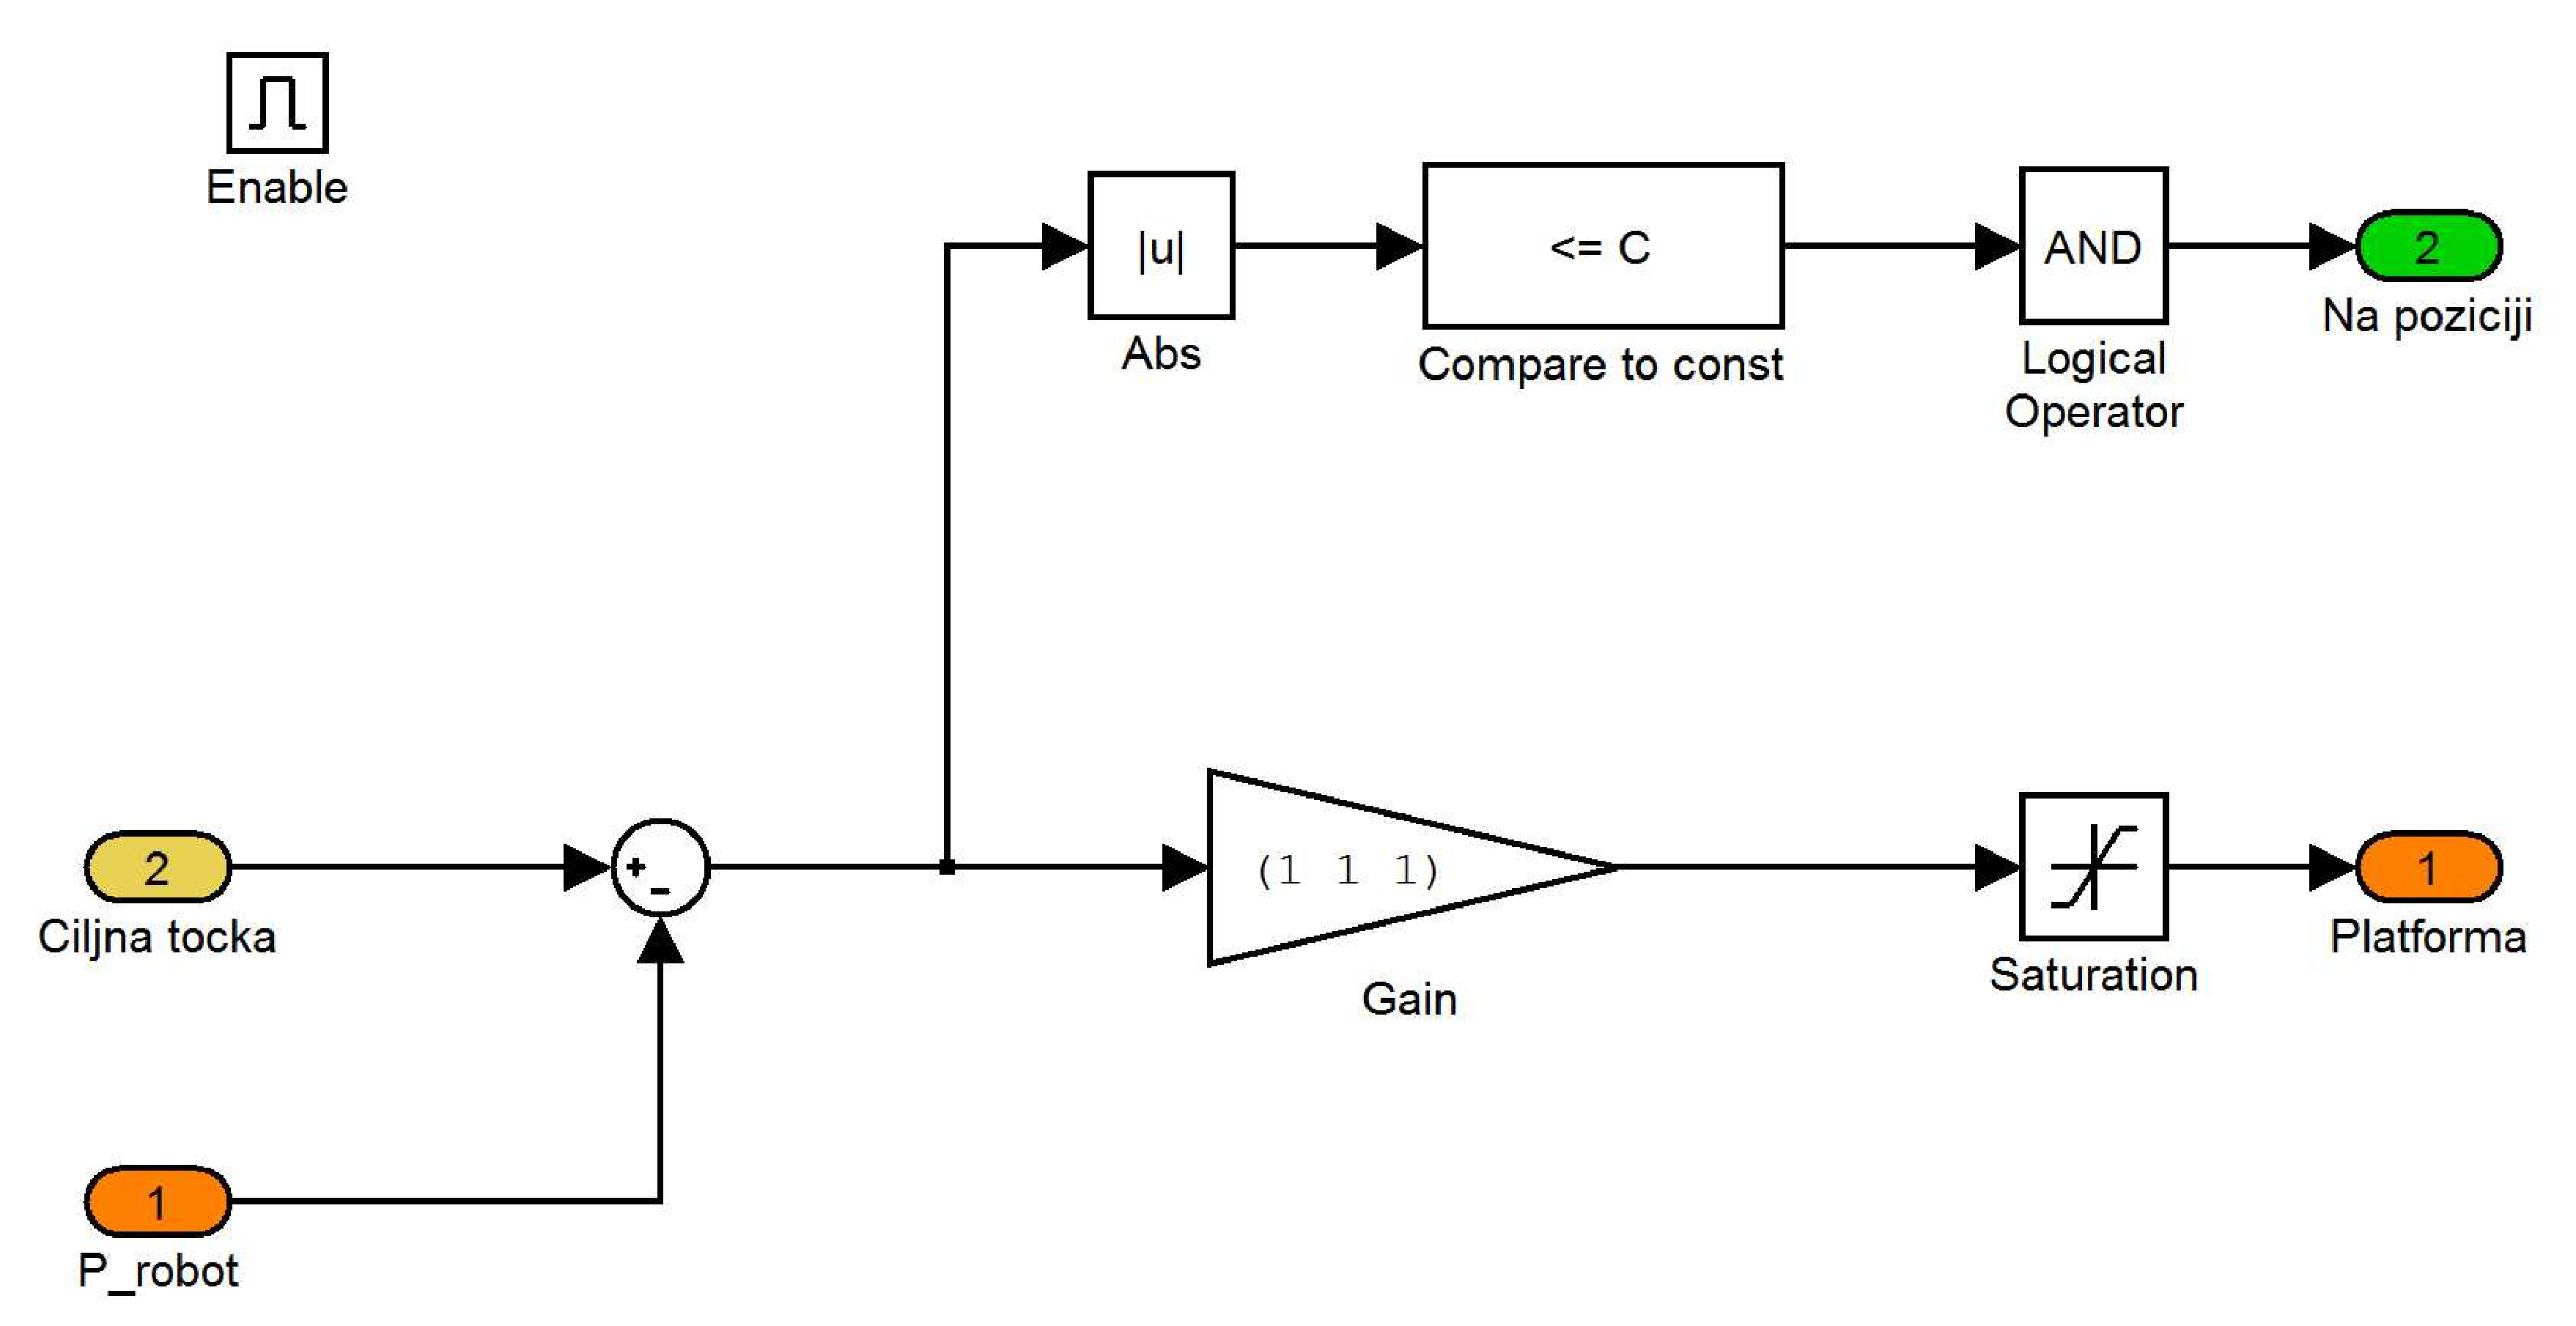
\includegraphics[draft=false]{PKrmilnik.eps}}
\caption{Slika prikazuje blok P-krmilnika.}
\label{fig:PKrmilnik}
\end{figure}



%\verb"if (abs(er(1))<erp && abs(er(2))<erp && abs(er(3))<erfi)" \newline
%\hspace*{1cm} \verb"pogoj = 1;"\newline
%\verb"else"\newline
%\hspace*{1cm} \verb"pogoj = 0;"\newline
%
%\begin{itemize}
%\item \verb"erp" - dovoljeno odstopanje za pozicijski del napake,
%\item \verb"erfi" - dovoljeno odstopanje za napake kota.
%\end{itemize}

\item \textbf{Vodenje platforme na izbrano točko.} V glavnem diagramu prehajanja stanj (blok \verb"Naloga") je potrebno dodati stanje 38 (Premakni platformo na točko Tx). Slika \ref{fig:DiagramNaTocko} prikazuje primer diagrama prehajanja stanj za premik platforme iz trenutne lege v željeno točko.

\begin{figure}[h]
\centering \resizebox{10cm}{!}{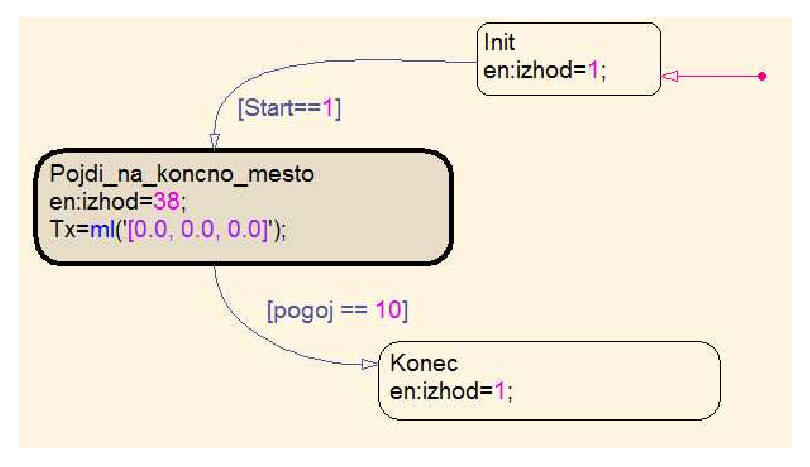
\includegraphics[draft=false]{DiagNaTocko.eps}}
\caption{Diagram prehajanja stanj za vodenje do točke $T_x=[0.0,0.0,0.0]$.}
\label{fig:DiagramNaTocko}
\end{figure}

\newpage



\item \textbf{Vodenje platforme do kocke.} Pri pobiranju kocke se mora paltforma pripeljati na točko, ki je dovolj blizu kocke, da jo lahko KUKA robotska roka pobere. Vsekakor pa platforme ne smemo poslati na točko, kjer se nahaja kocka, saj je koordinatni sistem platfomre postavljen na mesto, kjer se nahaja robotska roka in bi zato platforma premaknila kocko, ko bi se zadela vanjo. Razmere pojasnuje slika \ref{fig:KUKAKocka}.

\begin{mdframed}[backgroundcolor=yellow!20, shadow=true,roundcorner=8pt]

    Potrebno je torej določiti točko $T_x=[x_r,y_r,\varphi_r]$, tako da bo lahko KUKA robotska roka pobrala kocko. Razdalja med točko $T_k=[x_k,y_k,\varphi_k]$, kjer se nahaja kocka, ter točko $T_x=[x_r,y_r,\varphi_r]$, kamor se bo postavila platforma je $d=0.38$:

\begin{eqnarray}
    x_r = x_k-d\cdot cos(\varphi_k) \\
    y_r = y_k-d\cdot sin(\varphi_k) \\
    \varphi_r = \varphi_k
\end{eqnarray}

Orientacija KUKA platforma $\varphi_r$ je enaka orientaciji kocke $\varphi_k$.

Odprite blok \verb"Rutine/Pojdi_do_Tocke/Tk2Tr". Vanj vpišite enačbe za izračun točke v Matlab skriptnem jeziku.

\begin{itemize}
\item Vhod v blok je
\begin{itemize}
\item točka \verb"Tr", kjer se nahaja kocka in
\item parameter \verb"d", ki podaja oddaljenost KUKA platforme od kocke.
\end{itemize}
\item Izhod je točka \verb"Tr", ki je točka kamor naj se premakne robot.\\
\end{itemize}

V diagramu prehajanja stanj zamenjajte stanje 38 s stanjem 4 (Pojdi do zelene kocke).

\end{mdframed}

\begin{figure}[h]
\psfrag{xg}[][l][2.0][0]{$x_g$}
\psfrag{yg}[][l][2.0][0]{$y_g$}
\psfrag{xk}[][l][2.0][0]{$x_k$}
\psfrag{yk}[][l][2.0][0]{$y_k$}
\psfrag{xt}[][l][2.0][0]{$x_r$}
\psfrag{yt}[][l][2.0][0]{$y_r$}
\psfrag{xr}[][l][2.0][0]{$x_r$}
\psfrag{yr}[][l][2.0][0]{$y_r$}
\psfrag{dx}[][l][2.0][0]{$\Delta x$}
\psfrag{dy}[][l][2.0][0]{$\Delta y$}
\psfrag{d}[][l][2.0][0]{$d$}
\psfrag{thk}[][c][2.0][0]{$\varphi_k,\,\, \varphi_r$}
\centering \resizebox{10cm}{!}{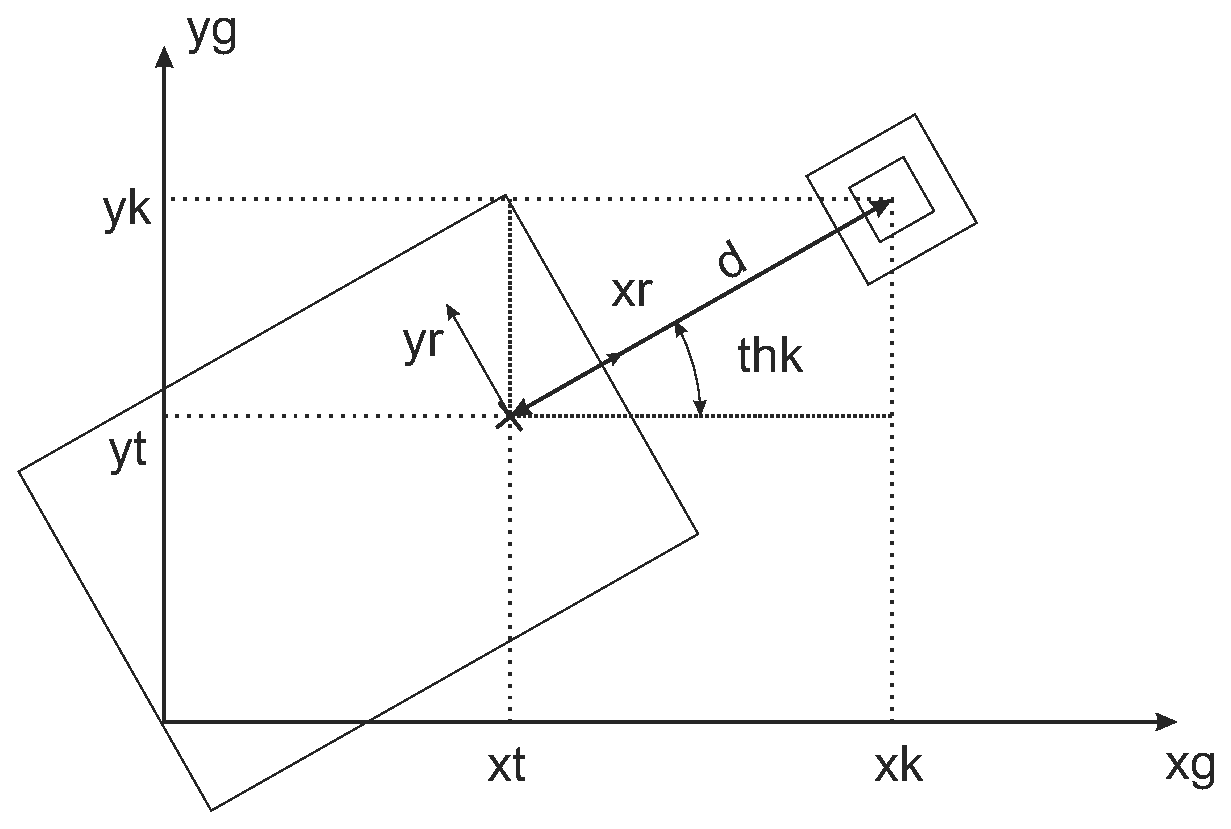
\includegraphics[draft=false]{KukaDoKocke.eps}}
\caption{Določanje točke za vodenje platforme pri pobiranju kocke.}
\label{fig:KUKAKocka}
\end{figure}

\end{enumerate}

\section{Naloga Hanojski stolp}

Ko vodenje KUKA platforme deluje pravilno, se lahko lotite priprave naloge Hanojski stolp. Celotna naloga je sestavljena iz naslednjih korakov:

\begin{figure}[h]
\psfrag{T1}[][][3.0][0]{$T_1$}
\psfrag{T10}[][][3.0][0]{$T_{10}$}
\psfrag{T2}[][][3.0][0]{$T_2$}
\psfrag{T3}[][][3.0][0]{$T_3$}
\psfrag{T4}[][][3.0][0]{$T_4$}
\psfrag{T5}[][][3.0][0]{$T_5$}
\psfrag{T6}[][][3.0][0]{$T_6$}
\psfrag{T7}[][][3.0][0]{$T_7$}
\psfrag{T8}[][][3.0][0]{$T_8$}
\psfrag{T9}[][][3.0][0]{$T_9$}
\psfrag{Z1}[][][3.0][0]{$Z_1$}
\psfrag{Rd1}[][][3.0][0]{$Rd_1$}
\psfrag{Rd2}[][][3.0][0]{$Rd_2$}
\psfrag{Ru1}[][][3.0][0]{$Ru_1$}
\psfrag{Ru2}[][][3.0][0]{$Ru_2$}
\psfrag{Ru3}[][][3.0][0]{$Ru_3$}
\psfrag{T4}[][][3.0][0]{$T_4$}
\psfrag{T5}[][][3.0][0]{$T_5$}
\psfrag{T6}[][][3.0][0]{$T_6$}
\psfrag{T7}[][][3.0][0]{$T_7$}
\psfrag{T8}[][][3.0][0]{$T_8$}
\psfrag{T9}[][][3.0][0]{$T_9$}
\psfrag{Odl1}[][][2.0][0]{Končo odlagališče}
\psfrag{Odl2}[][][2.0][0]{Vmesno odlagališče}
\psfrag{Odl3}[][][2.0][0]{Začetno odlagališče}
\psfrag{dol}[][l][3.0][0]{$wim$}
\psfrag{sir}[][l][3.0][0]{$him$}
\centering \resizebox{14cm}{!}{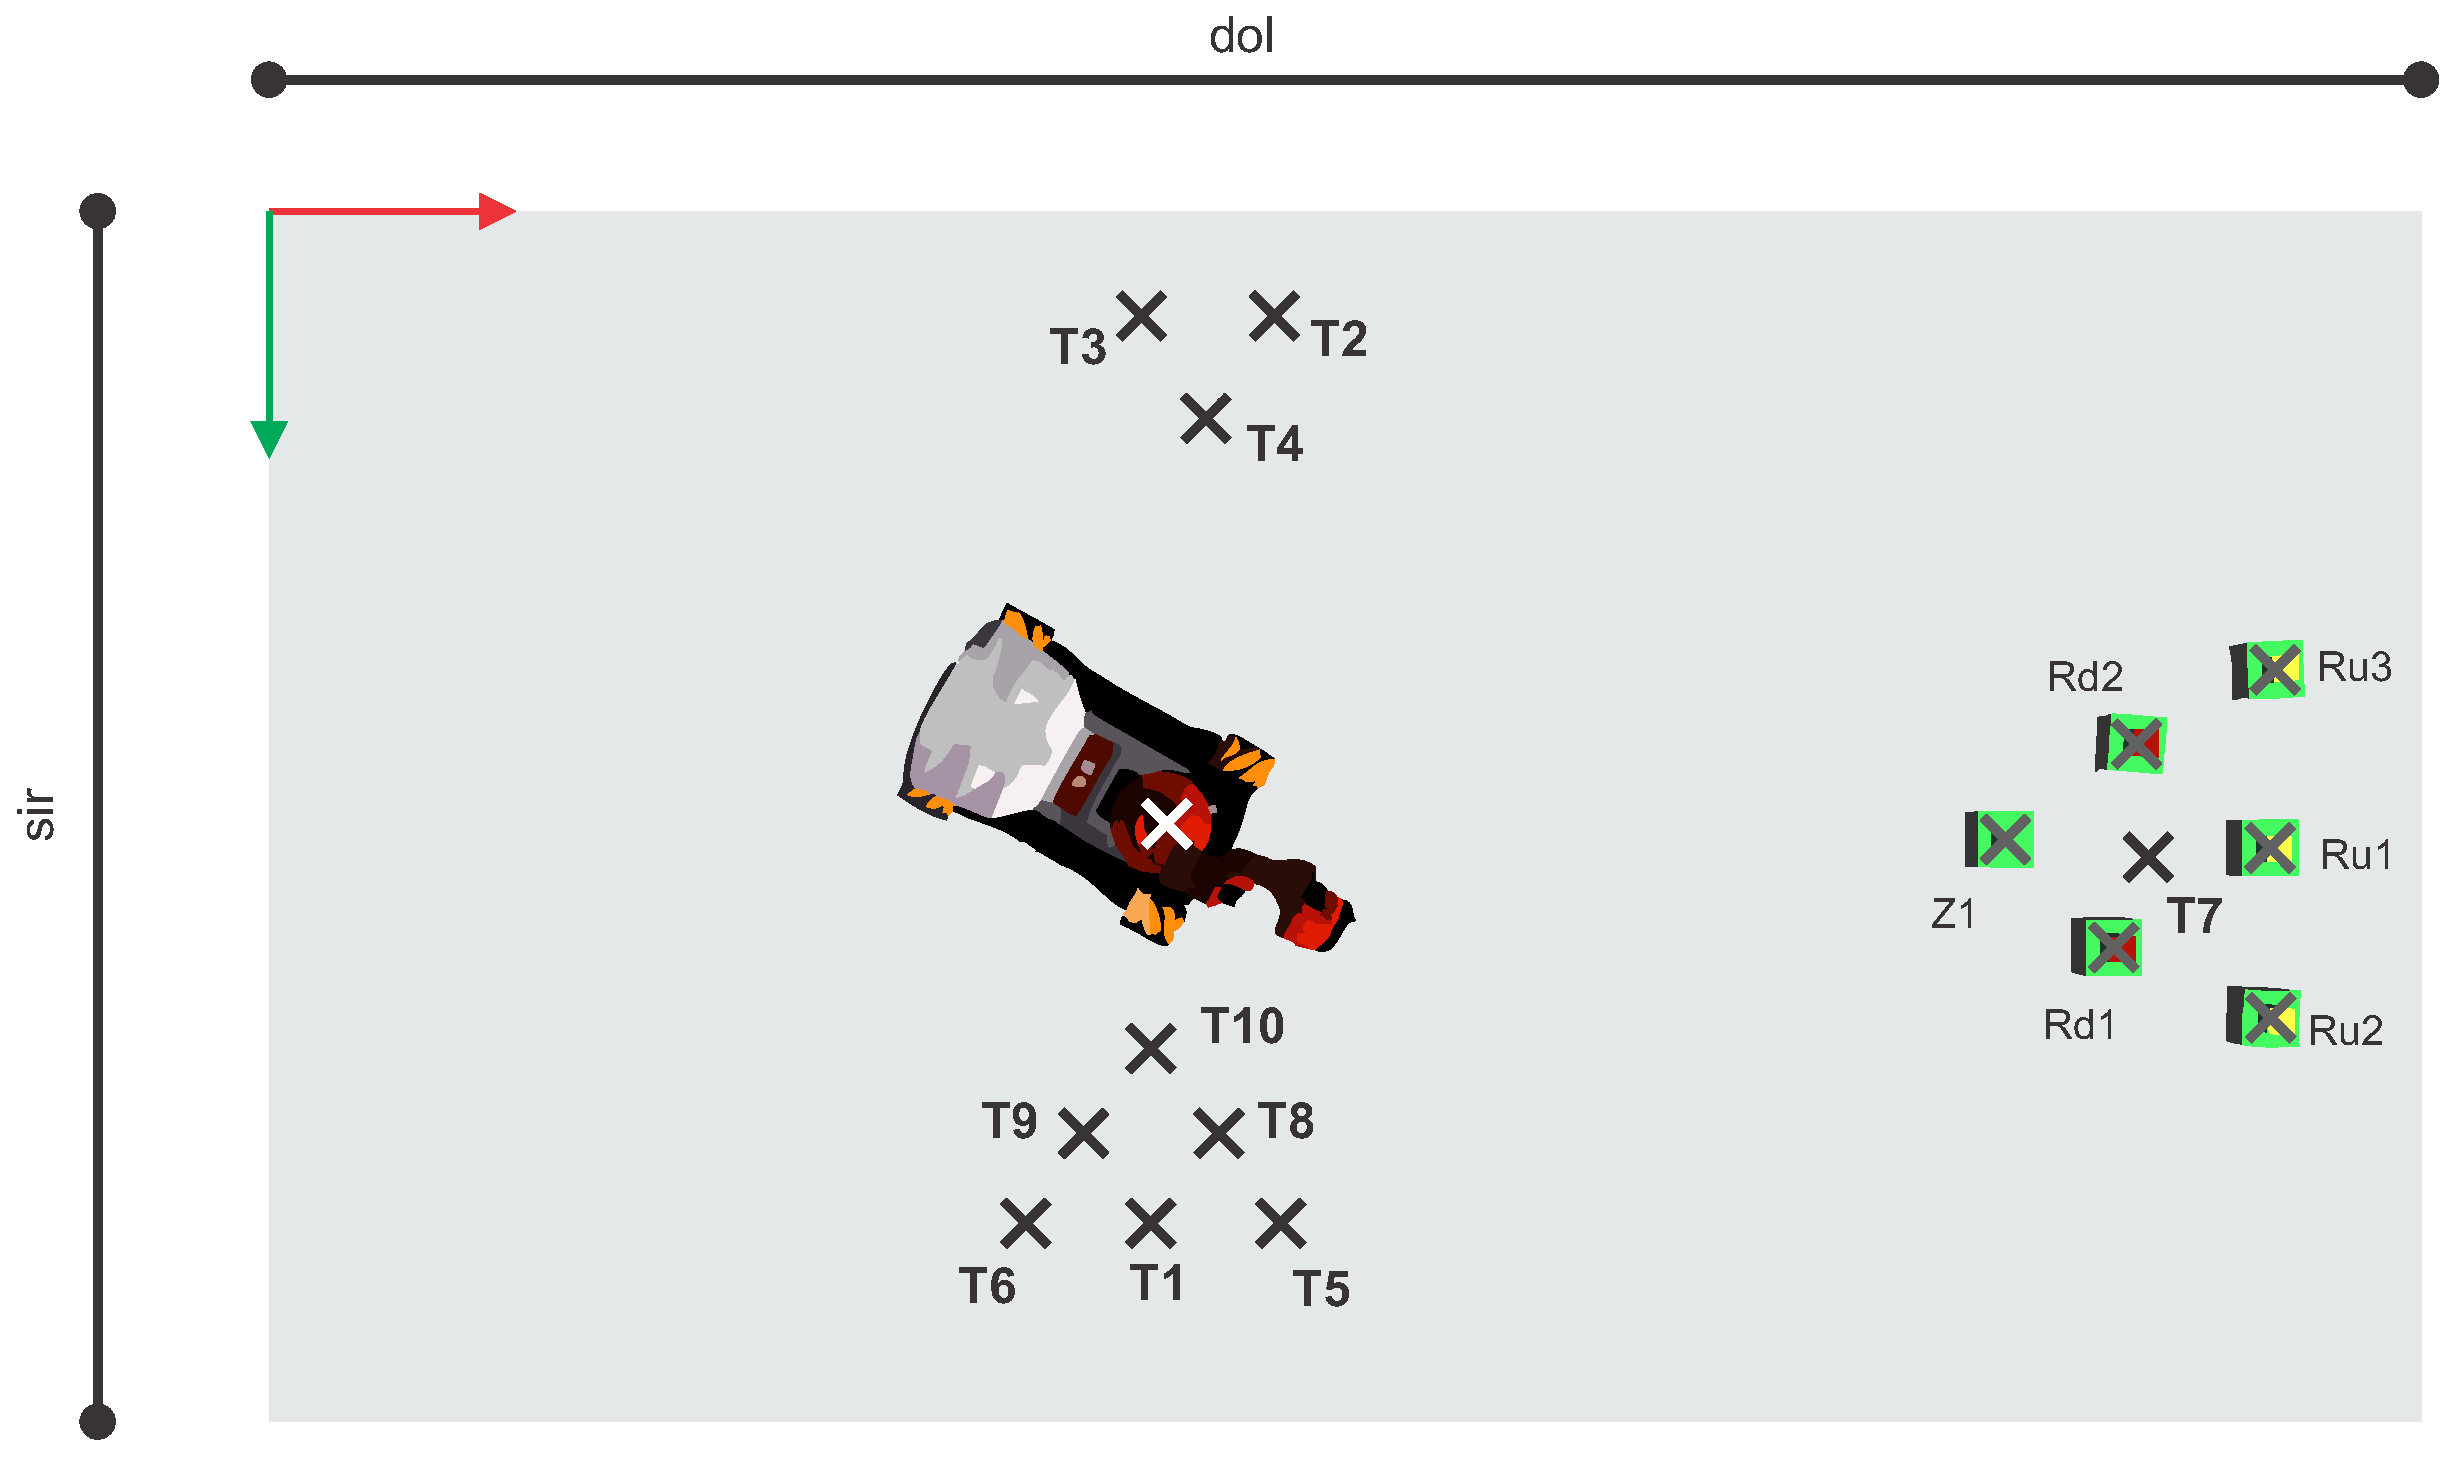
\includegraphics[draft=false]{tocke.eps}}
\caption{Posamezne točke v delovnem prostoru KUKA platforme.}
\label{fig:AllTocke}
\end{figure}


%\begin{enumerate}
%\item Zelena kocka na končno odlagališče.
%\item Rdeči kocki na vmesno odlagališče.
%\item Zelena kocka na vmesno odlagališče.
%\item Rumene kocke na koncno odlagališče.
%\item Zelena kocka na začetno odlagališče.
%\item Rdeči kocki na končno odlagališče.
%\item Zelena kocka na končno odlagališče.
%\end{enumerate}

\emph{Hanojski stolp} je logična igra. Najpreprostejša oblika stolpa je sestavljena iz treh odlagališč in treh diskov različnih velikosti. Na prvem začetnem odlagališču so diski postavljeni po velikosti z največjim diskom na dnu in najmanšim diskom na vrhu. Cilj je postaviti na končnem odlagališču isti stolp. Vsakič lahko prestavimo samo end disk in vedno le manjšega na večjega. Manjši disk lahko vedno postavimo na večjega. Na prazno mesto lahko postavimo disk katerekoli velikosti.

V našem primeru imamo tri "diske":
\begin{itemize}
\item Zelena kocka - najmanjši disk.
\item Rdeči kocki - srednji disk.
\item Rumene kocke - največji disk.
\end{itemize}

Ko igramo igro Hanojski stolp s KUKA platformo, torej premikamo skupino kock, ki predstavljajo en enoten disk. Vsakič moramo torej prestaviti celotno skupino kock:

\begin{itemize}
\item Zelena kocka - prestavimo eno samo kocko, ki je ves čas v prijemalu KUKA robotske roke.
\item Rdeči kocki - ena kocka je na odložišču, ki se nahaja za robotsko roko, druga v prijemalu.
\item Rumene kocke - dve kocki sta na odložišču levo in desno za robotsko roko, tretja je v prijemalu.
\end{itemize}

Cilj naloge je torej, da s pomočjo robota prestavimo kocke iz začetne na končno odložišče. Rumenih kock ne smemo nikoli postaviti pred rdeče oziroma zelene kocke, pravtako rdečih kock ne smemo nikoli prstaviti pred zelene kocke. Vedno smemo prestavljati samo kocke ene barve, ker predstavljajo en disk, v vrsti morajo seveda ležati le kocke istih barv. Pravilni vrstni red postavitve je prikazan na sliki \ref{fig:AllTocke}. V delovnem prostoru je na voljo 10 točk za odlaganje posameznih skupin kock.

V diagramu prehajanja stanj (blok \verb"Naloga") je potrebno v pravem vrstnem redu dodati stanja, ki jih izberete izmed stanj v tabeli \ref{tab:kodenalog}. Začnete s prestavljanjem zelene kocke, nato sledijo rdeče, itd ... Nalogo Hanojski stolp je možno rešiti v sedmih potezah, kar pomeni tudi sedem stanj. Cilj je dosežen, ko v pravem vrstnem redu na končnem odlagališču ležijo vse kocke. Pri načrtovanju potez si lahko pomagata s preprosto izvedbo igre, ki jo najdete na spletu, če vtipkate v spletni iskalnik iskalno geslo \verb|play hanoi tower|.